\chapter{Evaluaci\'{o}n y aplicaci\'{o}n de los modelos DL}

  Este cap\'{i}tulo abarca la evaluaci\'{o}n de los modelos de DL seleccionados en los pasos anteriores de la metodolog\'{i}a KDD. Para ello est\'{a}n definidas las m\'{e}tricas y algunos par\'{a}metros, no obstante, es necesario realizar unas primeras pruebas para terminar de ajustar los par\'{a}metros restantes. En las tablas obtenidas de los resultados se definen tres colores representativos, que va a permitir definir una superioridad o inferioridad de los algoritmos, estos colores son:
  \begin{itemize}
  	\item \colorbox{green}{Verde}: representa el valor m\'{a}s alto en la m\'{e}trica.
  	\item \colorbox{yellow}{Amarillo}: representa el segundo mejor valor de la m\'{e}trica.
  	\item \colorbox{red}{Rojo}: representa el peor valor de la m\'{e}trica.
  \end{itemize}

Ahora se procede a realizar los experimentos definidos para evaluar los algoritmos propuestos. Estos experimentos conforman la parte $8$ de la metodolog\'{i}a, centrada en la evaluaci\'{o}n de los modelos seleccionados.

\section{Experimento 1: Comparaci\'{o}n entre la selecci\'{o}n de datos para las pruebas}

Este primer experimento est\'{a} basado en buscar la mejor proporci\'{o}n de datos para el entrenamiento y prueba, para ello se usar\'{a} el algoritmo KNN de ML con los datos desbalanceados.

\begin{table}[h!]
	\begin{longtable}{|c|c|c|c|c|c|c|}
		\hline
		\%Test & Model & Accuracy & AUC & Precision& Recall & F1 \\ \hline
		10\% & KNN IMBALANCE & \colorbox{yellow}{0.997} & \colorbox{green}{0.571} & \colorbox{green}{1} & \colorbox{green}{0.14285714} & \colorbox{green}{0.25} \\ \hline
		20\% & KNN IMBALANCE & \colorbox{green}{0.99775} & \colorbox{yellow}{0.55} & \colorbox{green}{1} & \colorbox{yellow}{0.1} & \colorbox{yellow}{0.181818182}\\ \hline
		30\% & KNN IMBALANCE & 0.996833333 & 0.525 & \colorbox{green}{1} & 0.05 & 0.09523809523809523\\ \hline
		40\% & KNN IMBALANCE & \colorbox{red}{0.996375} & \colorbox{red}{0.5} & \colorbox{red}{0} & \colorbox{red}{0} & \colorbox{red}{0}\\ \hline
		50\% & KNN IMBALANCE & 0.9971 & \colorbox{red}{0.5}	& \colorbox{red}{0} & \colorbox{red}{0} & \colorbox{red}{0}\\ \hline
	\end{longtable}
	\caption{Puntuaci\'{o}n de tama\~{n}os de prueba en KNN desbalanceado.}
	\label{t:1}
\end{table}

\begin{figure}[h!]
	\centering
	\includegraphics[width=0.8\textwidth]{"figuras/Experimento1/KNN_Test_size"}
	\caption{Puntuaciones por tama\~{n}os de prueba en KNN desbalanceado.}
\end{figure}

Observaciones:
\begin{enumerate}
	\item Los peores resultados se obtienen cuando el por ciento de datos para la prueba es de 40\% y 50\% del conjunto de datos.
	\item El mejor resultado lo obtiene cuando el por ciento de datos para las pruebas es de un 10\% del conjunto de datos.
	\item La mejor exactitud de predicci\'{o}n es cuando se realiza la prueba con un 20\% del conjunto de datos.
\end{enumerate}

Por lo tanto, se decide tomar un 20\% de datos para realizar las pruebas, porque posee mayor exactitud y posee el segundo mejor resultado de \textit{F1 Score}, ya que con un 10\% se pierde exactitud en las predicciones a pesar de tener el mejor \textit{F1 Score}.

\section{Experimento 2: Comparaci\'{o}n entre los modelos de ML por estrategias para solucionar al desbalance de la informaci\'{o}n}

  El objetivo de este experimento es seleccionar los mejores modelos ML por estrategias. Para ello se utilizar\'{a}n los modelos DT, GNB, KNN, LR, MLP, RF y XGBOOST, y cada modelo se le aplicar\'{a}n las estrategias con datos desbalanceados, UnderSampler, OverSampler, SMOTE y ADASYN. Una vez definido los modelos y estrategias, se procede a realizar el experimento y obtener los resultados.
  
  \begin{longtable}{|c|c|c|c|c|c|}
  	\hline
  	Model & Accuracy & AUC & Precision & Recall & F1\\ \hline
  	\endfirsthead
  	\hline
  	Model & Accuracy & AUC & Precision & Recall & F1\\ \hline
  	\endhead
  	RF IMABALANCED & \colorbox{green}{0.99775} & 0.681567 & \colorbox{yellow}{0.666667} & 0.363636 & \colorbox{green}{0.470588}\\ \hline
  	XGBOOST IMBALANCED & \colorbox{yellow}{0.9975} & 	0.681442 & 0.571429 & 0.363636 & \colorbox{yellow}{0.444444}\\ \hline
  	KNN IMBALANCE & \colorbox{green}{0.99775} & 0.590909 & \colorbox{green}{1} & 0.181818 & 0.307692\\ \hline
  	DT IMBALANCED & 0.99425 & 0.679813 & 0.2 & 0.363636 & 0.258065\\ \hline
  	RF ADASYN & 0.997 & 0.583083 & 0.5 & 0.166667 & 0.25\\ \hline
  	RF OVERSAMPLE & 0.997 & 0.599499 & 0.333333 & 0.2 & 0.25\\ \hline
  	XGBOOST  & 0.9965 & 0.599248 & 0.25 & 0.2 & 0.222222\\ \hline
  	DT OVERSAMPLE & 0.99575 & 0.598872 & 0.181818 & 0.2 & 0.190476\\ \hline
  	RF SMOTE & 0.99675 & 0.535714 & \colorbox{green}{1} & 0.071429 & 0.133333\\ \hline
  	XGBOOST ADASYN  & 0.9925 & 0.580826 & 0.090909 & 0.166667 & 0.117647\\ \hline
  	NB IMBALANCED & 0.98 & \colorbox{green}{0.717997} & 0.063291 & 0.454545 & 0.111111\\ \hline
  	XGBOOST SMOTE & 0.99425 & 0.53446 & 0.090909 & 0.071429 & 0.08\\ \hline
  	LR ADASYN  & 0.986 & 0.577566 & 0.041667 & 0.166667 & 0.066667\\ \hline
  	NB UNDERSAMPLE & 0.96425 & \colorbox{yellow}{0.710101} & 0.035211 & 0.454545 & 0.065359\\ \hline
  	LR SMOTE & 0.98525 & 0.565533 & 0.040816 & 0.142857 & 0.063492\\ \hline
  	LR OVERSAMPLE & 0.9845 & 0.593233 & 0.035714 & 0.2 & 0.060606\\ \hline
  	NB ADASYN & 0.969 & 0.610582 & 0.025424 & 0.25 & 0.046154\\ \hline
  	DT SMOTE & 0.98575 & 0.530195 & 0.022222 & 0.071429 & 0.033898\\ \hline
  	MLP  ADASYN & 0.95275 & 0.602432 & 0.016393 & 0.25 & 0.030769\\ \hline
  	DT ADASYN & 0.9825 & 0.534269 & 0.016667 & 0.083333 & 0.027778\\ \hline
  	NB OVERSAMPLE & 0.96275 & 0.582331 & 0.013986 & 0.2 & 0.026144\\ \hline
  	MLP SMOTE & 0.95575 & 0.550731 & 0.011976 & 0.142857 & 0.022099\\ \hline
  	NB SMOTE & 0.972 & 0.523296 & 0.01 & 0.071429 & 0.017544\\ \hline
  	KNN SMOTE & 0.76225 & 0.595997 & 0.006322 & 0.428571 & 0.012461\\ \hline
  	RF UNDERSAMPLE & 0.724 & 0.634973 & 0.00543 & 0.545455 & 0.010753\\ \hline
  	KNN ADASYN & 0.806 & 0.570378 & 0.005181 & 0.333333 & 0.010204\\ \hline
  	DT UNDERSAMPLE & 0.586 & 0.611112 & 0.004219 & 0.636364 & 0.008383\\ \hline
  	XGBOOST UNDERSAMPLE & 0.32725 & 0.572039 & 0.003336 & \colorbox{green}{0.818182} & 0.006645\\ \hline
  	KNN UNDERSAMPLE & 0.57375 & 0.514312 & 0.002934 & 0.454545 & 0.005831\\ \hline
  	MLP UNDERSAMPLE & 0.03425 & 0.515793 & 0.002839 & \colorbox{green}{1} & 0.005663\\ \hline
  	LR UNDERSAMPLE & \colorbox{red}{0.00275} & 0.5 & 0.00275 & \colorbox{green}{1} & 0.005485\\ \hline
  	MLP OVERSAMPLE & 0.155 & \colorbox{red}{0.376942} & 0.001774 & 0.6 & 0.003538\\ \hline
  	MLP IMBALANCE & 0.99675 & 0.499749 & \colorbox{red}{0} & \colorbox{red}{0} & \colorbox{red}{0}\\ \hline
  	KNN OVERSAMPLE & 0.9915 & 0.496992 & \colorbox{red}{0} & \colorbox{red}{0} & \colorbox{red}{0}\\ \hline
  	LR IMBALANCED & 0.99725 & 0.5 & \colorbox{red}{0} & \colorbox{red}{0} & \colorbox{red}{0}\\ \hline
  	\caption{Puntuaciones de las pruebas de los modelos ML por estrategias.}
  	\label{t:2}
  \end{longtable}

Basados en la tabla \ref{t:2} y en los anexos ~\ref{an:1}, ~\ref{an:2}, ~\ref{an:3}, ~\ref{an:4} y ~\ref{an:5}, se pueden obtener las siguientes observaciones:

\begin{itemize}
	\item El modelo con mejor resultado es RF con datos desbalanceados.
	\item El segundo mejor resultado lo obtiene el modelo XGBOOST con datos desbalanceados.
	\item El peor resultado lo obtiene el modelo LR con datos desbalanceados.
	\item El mejor resultado en el modelo DT se obtiene con la estrategia OverSampler.
	\item El mejor resultado en el modelo KNN se obtiene con los datos desbalanceados.
	\item El mejor resultado en el modelo LR se obtiene con ADASYN.
	\item El mejor resultado en el modelo MPLClssifier se obtiene con ADASYN.
	\item El mejor resultado en el modelo NB se obtiene con datos desbalanceados.
	\item El mejor resultado en el modelo RF se obtiene con datos desbalanceados.
	\item El mejor resultado en el modelo XGBOOST se obtiene con datos desbalanceados.
	\item El mejor resultado con datos desbalanceados lo obtiene el modelo RF.
	\item El mejor resultado con UnderSampler lo obtiene el modelo NB.
	\item El mejor resultado con OverSampler lo obtiene el modelo RF.
	\item El mejor resultado con SMOTE lo obtiene el modelo RF.
	\item El mejor resultado con ADASYN lo obtiene el modelo RF.
	\item El modelo RF presenta superioridad con respecto a los dem\'{a}s modelos.
\end{itemize}

Con estas observaciones son suficientes para decidir los modelos que representar\'{a}n a los modelos ML. Se escoge el modelo RF con datos desbalanceados, OverSampler, SMOTE y ADASYN, y el modelo NB con UnderSampler para pr\'{o}ximos experimentos como los mejores modelos ML.

\section{Experimento 3: Comparaci\'{o}n en el orden de los \textit{dropout} con datos desbalanceados}

En este experimento se analizar\'{a} el orden los \textit{dropout} de los algoritmos CNN y RNN, donde el m\'{a}ximo posible recomendado por la librer\'{i}a es $0.5$. Se realizar\'{a}n las pruebas con datos desbalanceados y $1$ \textit{epoch} para los \'{o}rdenes de \textit{dropout} mostrados en la tabla.

	\begin{longtable}{|c|c|c|c|c|c|c|}
		\hline
		Dropout & Model & Accuracy & AUC & Precision & Recall & F1\\ \hline
		\endfirsthead
		\hline
		Dropout & Model & Accuracy & AUC & Precision & Recall & F1\\ \hline
		\endhead
		0.5-0.4-0.3 & CNN IMBALANCE & \colorbox{green}{0.999} & \colorbox{green}{0.714286} & \colorbox{green}{0.999001} & \colorbox{green}{0.999} & \colorbox{green}{0.9988}\\ \hline
		0.3-0.4-0.5 & CNN IMBALANCE & \colorbox{green}{0.999} & \colorbox{green}{0.714286} & \colorbox{green}{0.999001} & \colorbox{green}{0.999} & \colorbox{green}{0.9988}\\ \hline
		0.5-0.5-0.5 & CNN IMBALANCE & \colorbox{green}{0.999} & \colorbox{green}{0.714286} & \colorbox{green}{0.999001} & \colorbox{green}{0.999} & \colorbox{green}{0.9988}\\ \hline
		0.4-0.4-0.4 & CNN IMBALANCE & \colorbox{yellow}{0.99875} & \colorbox{yellow}{0.71416} & \colorbox{yellow}{0.998563} & \colorbox{yellow}{0.99875} & \colorbox{yellow}{0.99858}\\ \hline
		0.3-0.3-0.3 & CNN IMBALANCE & \colorbox{yellow}{0.99875} & \colorbox{yellow}{0.71416} & \colorbox{yellow}{0.998563} & \colorbox{yellow}{0.99875} & \colorbox{yellow}{0.99858}\\ \hline
		0.2-0.2-0.2 & CNN IMBALANCE & \colorbox{yellow}{0.99875} & \colorbox{yellow}{0.71416} & \colorbox{yellow}{0.998563} & \colorbox{yellow}{0.99875} & \colorbox{yellow}{0.99858}\\ \hline
		0.2-0.2-0.5 & CNN IMBALANCE & \colorbox{yellow}{0.99875} & \colorbox{yellow}{0.71416} & \colorbox{yellow}{0.998563} & \colorbox{yellow}{0.99875} & \colorbox{yellow}{0.99858}\\ \hline
		0.5-0.2-0.2 & CNN IMBALANCE & \colorbox{yellow}{0.99875} & \colorbox{yellow}{0.71416} & \colorbox{yellow}{0.998563} & \colorbox{yellow}{0.99875} & \colorbox{yellow}{0.99858}\\ \hline
		0.5-0.4-0.3 & RNN IMBALANCE & \colorbox{red}{0.99825} & \colorbox{red}{0.5} & \colorbox{red}{0.996503} & \colorbox{red}{0.99825} & \colorbox{red}{0.997376}\\ \hline
		0.3-0.4-0.5 & RNN IMBALANCE & \colorbox{red}{0.99825} & \colorbox{red}{0.5} & \colorbox{red}{0.996503} & \colorbox{red}{0.99825} & \colorbox{red}{0.997376}\\ \hline
		0.5-0.5-0.5 & RNN IMBALANCE & \colorbox{red}{0.99825} & \colorbox{red}{0.5} & \colorbox{red}{0.996503} & \colorbox{red}{0.99825} & \colorbox{red}{0.997376}\\ \hline
		0.4-0.4-0.4 & RNN IMBALANCE & \colorbox{red}{0.99825} & \colorbox{red}{0.5} & \colorbox{red}{0.996503} & \colorbox{red}{0.99825} & \colorbox{red}{0.997376}\\ \hline
		0.3-0.3-0.3 & RNN IMBALANCE & \colorbox{red}{0.99825} & \colorbox{red}{0.5} & \colorbox{red}{0.996503} & \colorbox{red}{0.99825} & \colorbox{red}{0.997376}\\ \hline
		0.2-0.2-0.2 & RNN IMBALANCE & \colorbox{red}{0.99825} & \colorbox{red}{0.5} & \colorbox{red}{0.996503} & \colorbox{red}{0.99825} & \colorbox{red}{0.997376}\\ \hline
		0.2-0.2-0.5 & RNN IMBALANCE & \colorbox{red}{0.99825} & \colorbox{red}{0.5} & \colorbox{red}{0.996503} & \colorbox{red}{0.99825} & \colorbox{red}{0.997376}\\ \hline
		0.5-0.2-0.2 & RNN IMBALANCE & \colorbox{red}{0.99825} & \colorbox{red}{0.5} & \colorbox{red}{0.996503} & \colorbox{red}{0.99825} & \colorbox{red}{0.997376}\\ \hline
		\caption{Puntuaci\'{o}n en las pruebas del modelo CNN con datos desbalanceados para los \'{o}rdenes de \textit{dropout}.}
		\label{t:3}
	\end{longtable}

\begin{figure}[h!]
	\centering
	\includegraphics[width=0.8\textwidth]{"figuras/Experimento3/CNN_dropouts_tests"}
	\caption{Puntuaciones en las pruebas del modelo CNN con datos desbalanceados por dropouts.}
	\label{ff:1}
\end{figure}

\begin{figure}[h!]
	\centering
	\includegraphics[width=0.8\textwidth]{"figuras/Experimento3/RNN_dropouts_tests"}
	\caption{Puntuaciones en las pruebas del modelo RNN con datos desbalanceados por dropouts.}
	\label{ff:2}
\end{figure}

Basados en la tabla \ref{t:3} y en las figuras \ref{ff:1} y \ref{ff:2}, se obtienen las siguientes observaciones generales:
\begin{itemize}
	\item Los mejores resultados se obtienen con CNN con los dropouts 0.5-0.4-0.3, 0.3-0.4-0.5 y 0.5-0.5-0.5.
	\item Los peores resultados se obtienen con RNN, siendo los resultados indistinguibles con cualquier orden de dropout.
	\item El peor resultado con CNN es con los restantes \'{o}rdenes de dropouts, siendo sus resultados iguales.
	\item Los CNN dominan a RNN en cualquier orden de dropout.
\end{itemize}

Teniendo en cuenta esto, se decide usar de entre los 3 mejores dropouts, el orden 0.5-0.4-0.3 para los pr\'{o}ximos experimentos

\section{Experimento 4: Comparaci\'{o}n en los modelos DL teniendo en cuenta los resultados de las pruebas.}

  Este experimento est\'{a} orientado a seleccionar los mejores modelos DL teniendo en cuenta dos factores: la cantidad de \textit{epochs} de entrenamiento y la estrategia aplicada para la soluci\'{o}n al desbalance de la informaci\'{o}n. Para ello este experimento se dividir\'{a} en dos partes: primero, se analizar\'{a}n todos los modelos por \textit{epochs} y con la misma estrategia aplicada, segundo, se analizar\'{a}n todas las estrategias y \textit{epoch} por modelo. Luego de obtener las observaciones por cada una de las dos partes anteriores, se proceder\'{a} a obtener las observaciones generales y junto a ello, los mejores modelos en cuanto a las pruebas.
  
  Para el experimento se tiene en cuenta que: las cantidades de \textit{epochs} son $1$, $20$, $50$ y $100$, las estrategias son datos desbalanceados, UnderSampler, OverSampler, SMOTE y ADASYN, y los modelos a analizar son CNN, AE, DAE, RNN, LSTM y BPNN. Una vez definidas las bases del experimento, se proceden a realizar el experimento y analizarlo por cada una de las partes.

\subsection{Primera parte: Modelos por epochs con la misma estrategia.}

  Los resultados obtenidos se muestran a continuaci\'{o}n, para ello se dividir\'{a} por estrategias:
  
  \subsubsection{Datos desbalanceados}
  	\begin{longtable}{|c|c|c|c|c|c|c|}
  		\hline
  		Epoch & Model & Accuracy & AUC & Precision & Recall & F1\\ \hline
  		\endfirsthead
  		\hline
  		Epoch & Model & Accuracy & AUC & Precision & Recall & F1\\ \hline
  		\endhead
  		1 & CNN IMBALANCE & \colorbox{green}{0.99675} & \colorbox{green}{0.56666667} & \colorbox{green}{0.99676057} & \colorbox{green}{0.99675} & \colorbox{green}{0.99551}\\ \hline
  		50 & CNN IMBALANCE & \colorbox{green}{0.99675} & \colorbox{green}{0.56666667} & \colorbox{green}{0.99676057} & \colorbox{green}{0.99675} & \colorbox{green}{0.99551}\\ \hline
  		20 & CNN IMBALANCE & \colorbox{yellow}{0.9965} & \colorbox{yellow}{0.5665412} & 0.99550976 & \colorbox{yellow}{0.9965} & \colorbox{yellow}{0.99533596}\\ \hline
  		100 & CNN IMBALANCE & \colorbox{red}{0.99625} & 0.56641573 & 0.99488395 & \colorbox{red}{0.99625} & 0.99516706\\ \hline
  		1 & BPNN IMBALANCE & \colorbox{red}{0.99625} & \colorbox{red}{0.5} & \colorbox{yellow}{0.99626406} & \colorbox{red}{0.99625} & \colorbox{red}{0.99437852}\\ \hline
  		20 & BPNN IMBALANCE & \colorbox{red}{0.99625} & \colorbox{red}{0.5} & \colorbox{yellow}{0.99626406} & \colorbox{red}{0.99625} & \colorbox{red}{0.99437852}\\ \hline
  		50 & BPNN IMBALANCE & \colorbox{red}{0.99625} & \colorbox{red}{0.5} & \colorbox{yellow}{0.99626406} & \colorbox{red}{0.99625} & \colorbox{red}{0.99437852}\\ \hline
  		100 & BPNN IMBALANCE & \colorbox{red}{0.99625} & \colorbox{red}{0.5} & \colorbox{yellow}{0.99626406} & \colorbox{red}{0.99625} & \colorbox{red}{0.99437852}\\ \hline
  		1 & AE IMBALANCE & \colorbox{red}{0.99625} & \colorbox{red}{0.5} & \colorbox{red}{0.99251406} & \colorbox{red}{0.99625} & \colorbox{red}{0.99437852}\\ \hline
  		1 & DAE IMBALANCE & \colorbox{red}{0.99625} & \colorbox{red}{0.5} & \colorbox{red}{0.99251406} & \colorbox{red}{0.99625} & \colorbox{red}{0.99437852}\\ \hline
  		1 & RNN IMBALANCE & \colorbox{red}{0.99625} & \colorbox{red}{0.5} & \colorbox{red}{0.99251406} & \colorbox{red}{0.99625} & \colorbox{red}{0.99437852}\\ \hline
  		1 & LSTM IMBALANCE & \colorbox{red}{0.99625} & \colorbox{red}{0.5} & \colorbox{red}{0.99251406} & \colorbox{red}{0.99625} & \colorbox{red}{0.99437852}\\ \hline
  		20 & AE IMBALANCE & \colorbox{red}{0.99625} & \colorbox{red}{0.5} & \colorbox{red}{0.99251406} & \colorbox{red}{0.99625} & \colorbox{red}{0.99437852}\\ \hline
  		20 & DAE IMBALANCE & \colorbox{red}{0.99625} & \colorbox{red}{0.5} & \colorbox{red}{0.99251406} & \colorbox{red}{0.99625} & \colorbox{red}{0.99437852}\\ \hline
  		20 & RNN IMBALANCE & \colorbox{red}{0.99625} & \colorbox{red}{0.5} & \colorbox{red}{0.99251406} & \colorbox{red}{0.99625} & \colorbox{red}{0.99437852}\\ \hline
  		20 & LSTM IMBALANCE & \colorbox{red}{0.99625} & \colorbox{red}{0.5} & \colorbox{red}{0.99251406} & \colorbox{red}{0.99625} & \colorbox{red}{0.99437852}\\ \hline
  		50 & AE IMBALANCE & \colorbox{red}{0.99625} & \colorbox{red}{0.5} & \colorbox{red}{0.99251406} & \colorbox{red}{0.99625} & \colorbox{red}{0.99437852}\\ \hline
  		50 & DAE IMBALANCE & \colorbox{red}{0.99625} & \colorbox{red}{0.5} & \colorbox{red}{0.99251406} & \colorbox{red}{0.99625} & \colorbox{red}{0.99437852}\\ \hline
  		50 & RNN IMBALANCE & \colorbox{red}{0.99625} & \colorbox{red}{0.5} & \colorbox{red}{0.99251406} & \colorbox{red}{0.99625} & \colorbox{red}{0.99437852}\\ \hline
  		50 & LSTM IMBALANCE & \colorbox{red}{0.99625} & \colorbox{red}{0.5} & \colorbox{red}{0.99251406} & \colorbox{red}{0.99625} & \colorbox{red}{0.99437852}\\ \hline
  		100 & AE IMBALANCE & \colorbox{red}{0.99625} & \colorbox{red}{0.5} & \colorbox{red}{0.99251406} & \colorbox{red}{0.99625} & \colorbox{red}{0.99437852}\\ \hline
  		100 & DAE IMBALANCE & \colorbox{red}{0.99625} & \colorbox{red}{0.5} & \colorbox{red}{0.99251406} & \colorbox{red}{0.99625} & \colorbox{red}{0.99437852}\\ \hline
  		100 & RNN IMBALANCE & \colorbox{red}{0.99625} & \colorbox{red}{0.5} & \colorbox{red}{0.99251406} & \colorbox{red}{0.99625} & \colorbox{red}{0.99437852}\\ \hline
  		100 & LSTM IMBALANCE & \colorbox{red}{0.99625} & \colorbox{red}{0.5} & \colorbox{red}{0.99251406} & \colorbox{red}{0.99625} & \colorbox{red}{0.99437852}\\ \hline
  		\caption{Puntuaciones en las pruebas de los modelos DL con datos desbalanceados en 1, 20, 50 y 100 epochs.}
  		\label{t:4}
  	\end{longtable}

Basados en la tabla \ref{t:4} se obitenen las siguientes observaciones:
\begin{itemize}
	\item El mejor modelo es CNN con 1 y 50 \textit{epochs} con los mejores resultados.
	\item El segundo mejor modelo es CNN con 20 \textit{epochs} con los segundos mejores resultados a excepci\'{o}n de la precisi\'{o}n.
	\item Los peores modelos son AE, DAE, RNN y LSTM con los resultados id\'{e}nticos y los peores.
	\item La superioridad de modelos sin tener en cuenta la cantidad de \textit{epochs} es: CNN, BPNN y el resto en tercer lugar.
	\item Los resultados del modelo BPNN se comportas igual sin importar la cantidad de \textit{epochs}.
\end{itemize}

\subsubsection{UnderSampler}
\begin{longtable}{|c|c|c|c|c|c|c|}
	\hline
	Epoch & Model & Accuracy & AUC & Precision & Recall & F1\\ \hline
	\endfirsthead
	\hline
	Epoch & Model & Accuracy & AUC & Precision & Recall & F1\\ \hline
	\endhead
	1 & BPNN UNDERSAMPLE & \colorbox{green}{0.99625} & 0.5 & \colorbox{yellow}{0.99626406} & \colorbox{green}{0.99625} & \colorbox{green}{0.99437852}\\ \hline
	20 & BPNN UNDERSAMPLE & \colorbox{green}{0.99625} & 0.5 & \colorbox{yellow}{0.99626406} & \colorbox{green}{0.99625} & \colorbox{green}{0.99437852}\\ \hline
	50 & BPNN UNDERSAMPLE & \colorbox{green}{0.99625} & 0.5 & \colorbox{yellow}{0.99626406} & \colorbox{green}{0.99625} & \colorbox{green}{0.99437852}\\ \hline
	100 & BPNN UNDERSAMPLE & \colorbox{green}{0.99625} & 0.5 & \colorbox{yellow}{0.99626406} & \colorbox{green}{0.99625} & \colorbox{green}{0.99437852}\\ \hline
	1 & AE UNDERSAMPLE & \colorbox{green}{0.99625} & 0.5 & 0.99251406 & \colorbox{green}{0.99625} & \colorbox{green}{0.99437852}\\ \hline
	1 & DAE UNDERSAMPLE & \colorbox{green}{0.99625} & 0.5 & 0.99251406 & \colorbox{green}{0.99625} & \colorbox{green}{0.99437852}\\ \hline
	1 & RNN UNDERSAMPLE & \colorbox{green}{0.99625} & 0.5 & 0.99251406 & \colorbox{green}{0.99625} & \colorbox{green}{0.99437852}\\ \hline
	1 & LSTM UNDERSAMPLE & \colorbox{green}{0.99625} & 0.5 & 0.99251406 & \colorbox{green}{0.99625} & \colorbox{green}{0.99437852}\\ \hline
	20 & AE UNDERSAMPLE & \colorbox{green}{0.99625} & 0.5 & 0.99251406 & \colorbox{green}{0.99625} & \colorbox{green}{0.99437852}\\ \hline
	20 & DAE UNDERSAMPLE & \colorbox{green}{0.99625} & 0.5 & 0.99251406 & \colorbox{green}{0.99625} & \colorbox{green}{0.99437852}\\ \hline
	20 & RNN UNDERSAMPLE & \colorbox{green}{0.99625} & 0.5 & 0.99251406 & \colorbox{green}{0.99625} & \colorbox{green}{0.99437852}\\ \hline
	20 & LSTM UNDERSAMPLE & \colorbox{green}{0.99625} & 0.5 & 0.99251406 & \colorbox{green}{0.99625} & \colorbox{green}{0.99437852}\\ \hline
	50 & AE UNDERSAMPLE & \colorbox{green}{0.99625} & 0.5 & 0.99251406 & \colorbox{green}{0.99625} & \colorbox{green}{0.99437852}\\ \hline
	50 & DAE UNDERSAMPLE & \colorbox{green}{0.99625} & 0.5 & 0.99251406 & \colorbox{green}{0.99625} & \colorbox{green}{0.99437852}\\ \hline
	50 & RNN UNDERSAMPLE & \colorbox{green}{0.99625} & 0.5 & 0.99251406 & \colorbox{green}{0.99625} & \colorbox{green}{0.99437852}\\ \hline
	50 & LSTM UNDERSAMPLE & \colorbox{green}{0.99625} & 0.5 & 0.99251406 & \colorbox{green}{0.99625} & \colorbox{green}{0.99437852}\\ \hline
	100 & AE UNDERSAMPLE & \colorbox{green}{0.99625} & 0.5 & 0.99251406 & \colorbox{green}{0.99625} & \colorbox{green}{0.99437852}\\ \hline
	100 & DAE UNDERSAMPLE & \colorbox{green}{0.99625} & 0.5 & 0.99251406 & \colorbox{green}{0.99625} & \colorbox{green}{0.99437852}\\ \hline
	100 & RNN UNDERSAMPLE & \colorbox{green}{0.99625} & 0.5 & 0.99251406 & \colorbox{green}{0.99625} & \colorbox{green}{0.99437852}\\ \hline
	100 & LSTM UNDERSAMPLE & \colorbox{green}{0.99625} & 0.5 & 0.99251406 & \colorbox{green}{0.99625} & \colorbox{green}{0.99437852}\\ \hline
	100 & CNN UNDERSAMPLE & \colorbox{yellow}{0.76675} & \colorbox{green}{0.61727311} & 0.99368038 & \colorbox{yellow}{0.76675} & \colorbox{yellow}{0.86451737}\\ \hline
	50 & CNN UNDERSAMPLE & 0.53675 & 0.5350481 & 0.99301653 & 0.53675 & 0.69518094\\ \hline
	20 & CNN UNDERSAMPLE & 0.121 & \colorbox{red}{0.45922208} & \colorbox{red}{0.98997066} & 0.121 & 0.21089089\\ \hline
	1 & CNN UNDERSAMPLE & \colorbox{red}{0.0765} & \colorbox{yellow}{0.53651192} & \colorbox{green}{0.99626517} & \colorbox{red}{0.0765} & \colorbox{red}{0.13562832}\\ \hline
	\caption{Puntuaciones en las pruebas de los modelos DL con UnderSampler en 1, 20, 50 y 100 epochs.}
	\label{t:5}
\end{longtable}

Basados en la tabla \ref{t:5} se obtienen las siguientes observaciones:
\begin{itemize}
	\item El mejor modelo es BPNN en $1$, $20$, $50$ y $100$ con los mejores resultados a excepci\'{o}n de la precisi\'{o}n con los segundos mejores resultados y \textit{AUC Score}.
	\item Los segundos mejores modelos son AE, DAE, RNN y LSTM en $1$, $20$, $50$ y $100$ \textit{epochs} con resultados id\'{e}nticos a BPNN a diferencia de la precisi\'{o}n donde obtiene resultados m\'{a}s bajos.
	\item El peor modelo es CNN con $1$ \textit{epoch} con los peores resultados a excepci\'{o}n de \textit{AUC Score} con el segundo mejor resultado y la precisi\'{o}n con el mejor resultado.
	\item Los modelos AE, DAE, RNN y LSTM no presentan comportamientos diferentes en cuanto a los resultados sin importar el n\'{u}mero de \textit{epochs}.
\end{itemize}

\subsubsection{OverSampler}
\begin{longtable}{|c|c|c|c|c|c|c|}
	\hline
	Epoch & Model & Accuracy & AUC & Precision & Recall & F1\\ \hline
	\endfirsthead
	\hline
	Epoch & Model & Accuracy & AUC & Precision & Recall & F1\\ \hline
	\endhead
	1 & BPNN OVERSAMPLE & \colorbox{green}{0.99575} & \colorbox{red}{0.5} & \colorbox{green}{0.99576806} & \colorbox{green}{0.99575} & \colorbox{green}{0.99362953}\\ \hline
	20 & BPNN OVERSAMPLE & \colorbox{green}{0.99575} & \colorbox{red}{0.5} & \colorbox{green}{0.99576806} & \colorbox{green}{0.99575} & \colorbox{green}{0.99362953}\\ \hline
	50 & BPNN OVERSAMPLE & \colorbox{green}{0.99575} & \colorbox{red}{0.5} & \colorbox{green}{0.99576806} & \colorbox{green}{0.99575} & \colorbox{green}{0.99362953}\\ \hline
	100 & BPNN OVERSAMPLE & \colorbox{green}{0.99575} & \colorbox{red}{0.5} & \colorbox{green}{0.99576806} & \colorbox{green}{0.99575} & \colorbox{green}{0.99362953}\\ \hline
	1 & AE OVERSAMPLE & \colorbox{green}{0.99575} & \colorbox{red}{0.5} & \colorbox{red}{0.99151806} & \colorbox{green}{0.99575} & \colorbox{green}{0.99362953}\\ \hline
	1 & DAE OVERSAMPLE & \colorbox{green}{0.99575} & \colorbox{red}{0.5} & \colorbox{red}{0.99151806} & \colorbox{green}{0.99575} & \colorbox{green}{0.99362953}\\ \hline
	1 & RNN OVERSAMPLE & \colorbox{green}{0.99575} & \colorbox{red}{0.5} & \colorbox{red}{0.99151806} & \colorbox{green}{0.99575} & \colorbox{green}{0.99362953}\\ \hline
	1 & LSTM OVERSAMPLE & \colorbox{green}{0.99575} & \colorbox{red}{0.5} & \colorbox{red}{0.99151806} & \colorbox{green}{0.99575} & \colorbox{green}{0.99362953}\\ \hline
	20 & AE OVERSAMPLE & \colorbox{green}{0.99575} & \colorbox{red}{0.5} & \colorbox{red}{0.99151806} & \colorbox{green}{0.99575} & \colorbox{green}{0.99362953}\\ \hline
	20 & DAE OVERSAMPLE & \colorbox{green}{0.99575} & \colorbox{red}{0.5} & \colorbox{red}{0.99151806} & \colorbox{green}{0.99575} & \colorbox{green}{0.99362953}\\ \hline
	20 & RNN OVERSAMPLE & \colorbox{green}{0.99575} & \colorbox{red}{0.5} & \colorbox{red}{0.99151806} & \colorbox{green}{0.99575} & \colorbox{green}{0.99362953}\\ \hline
	20 & LSTM OVERSAMPLE & \colorbox{green}{0.99575} & \colorbox{red}{0.5} & \colorbox{red}{0.99151806} & \colorbox{green}{0.99575} & \colorbox{green}{0.99362953}\\ \hline
	50 & AE OVERSAMPLE & \colorbox{green}{0.99575} & \colorbox{red}{0.5} & \colorbox{red}{0.99151806} & \colorbox{green}{0.99575} & \colorbox{green}{0.99362953}\\ \hline
	50 & DAE OVERSAMPLE & \colorbox{green}{0.99575} & \colorbox{red}{0.5} & \colorbox{red}{0.99151806} & \colorbox{green}{0.99575} & \colorbox{green}{0.99362953}\\ \hline
	50 & RNN OVERSAMPLE & \colorbox{green}{0.99575} & \colorbox{red}{0.5} & \colorbox{red}{0.99151806} & \colorbox{green}{0.99575} & \colorbox{green}{0.99362953}\\ \hline
	50 & LSTM OVERSAMPLE & \colorbox{green}{0.99575} & \colorbox{red}{0.5} & \colorbox{red}{0.99151806} & \colorbox{green}{0.99575} & \colorbox{green}{0.99362953}\\ \hline
	100 & AE OVERSAMPLE & \colorbox{green}{0.99575} & \colorbox{red}{0.5} & \colorbox{red}{0.99151806} & \colorbox{green}{0.99575} & \colorbox{green}{0.99362953}\\ \hline
	100 & DAE OVERSAMPLE & \colorbox{green}{0.99575} & \colorbox{red}{0.5} & \colorbox{red}{0.99151806} & \colorbox{green}{0.99575} & \colorbox{green}{0.99362953}\\ \hline
	100 & RNN OVERSAMPLE & \colorbox{green}{0.99575} & \colorbox{red}{0.5} & \colorbox{red}{0.99151806} & \colorbox{green}{0.99575} & \colorbox{green}{0.99362953}\\ \hline
	100 & LSTM OVERSAMPLE & \colorbox{green}{0.99575} & \colorbox{red}{0.5} & \colorbox{red}{0.99151806} & \colorbox{green}{0.99575} & \colorbox{green}{0.99362953}\\ \hline
	100 & CNN OVERSAMPLE & \colorbox{yellow}{0.9875} & \colorbox{yellow}{0.70086101} & \colorbox{yellow}{0.99386401} & \colorbox{yellow}{0.9875} & \colorbox{yellow}{0.99040606}\\ \hline
	50 & CNN OVERSAMPLE & 0.9865 & 0.70035888 & 0.99381181 & 0.9865 & 0.98984607\\ \hline
	20 & CNN OVERSAMPLE & 0.98475 & 0.69948014 & 0.99373693 & 0.98475 & 0.98887889\\ \hline
	1 & CNN OVERSAMPLE & \colorbox{red}{0.93125} & \colorbox{green}{0.7019022} & 0.99346889 & \colorbox{red}{0.93125} & \colorbox{red}{0.9604627}\\ \hline
	\caption{Puntuaciones en las pruebas de los modelos DL con OverSampler en 1, 20, 50 y 100 epochs.}
	\label{t:6}
\end{longtable}

Basados en la tabla \ref{t:6} se obitenen las siguietnes observaciones:
\begin{itemize}
	\item El mejor modelo es BPNN en $1$, $20$, $50$ y $100$ \textit{epochs} con resultados id\'{e}nticos y los mejores a excepci\'{o}n de \textit{AUC Score} que obtiene el peor resultado.
	\item Los segundos mejores modelos son AE, DAE, RNN y LSTM con resultados id\'{e}nticos a BPNN a excepci\'{o}n de la precisi\'{o}n donde obtienen los peores resultados.
	\item El peor modelo es CNN en $1$ \textit{epoch} donde obtiene los peores resultados a excepci\'{o}n de \textit{AUC Score} con el mejor resultado y la precisi\'{o}n.
	\item Los resultados de los modelos AE, DAE, RNN y LSTM se comportan iguales sin importar la cantidad de \textit{epochs}.
\end{itemize}

\subsubsection{SMOTE}
\begin{longtable}{|c|c|c|c|c|c|c|}
	\hline
	Epoch & Model & Accuracy & AUC & Precision & Recall & F1\\ \hline
	\endfirsthead
	\hline
	Epoch & Model & Accuracy & AUC & Precision & Recall & F1\\ \hline
	\endhead
	1 & BPNN SMOTE & \colorbox{green}{0.9955} & \colorbox{red}{0.5} & \colorbox{green}{0.99552025} & \colorbox{green}{0.9955} & \colorbox{green}{0.99325507}\\ \hline
	20 & BPNN SMOTE & \colorbox{green}{0.9955} & \colorbox{red}{0.5} & \colorbox{green}{0.99552025} & \colorbox{green}{0.9955} & \colorbox{green}{0.99325507}\\ \hline
	50 & BPNN SMOTE & \colorbox{green}{0.9955} & \colorbox{red}{0.5} & \colorbox{green}{0.99552025} & \colorbox{green}{0.9955} & \colorbox{green}{0.99325507}\\ \hline
	100 & BPNN SMOTE & \colorbox{green}{0.9955} & \colorbox{red}{0.5} & \colorbox{green}{0.99552025} & \colorbox{green}{0.9955} & \colorbox{green}{0.99325507}\\ \hline
	1 & AE SMOTE & \colorbox{green}{0.9955} & \colorbox{red}{0.5} & \colorbox{red}{0.99102025} & \colorbox{green}{0.9955} & \colorbox{green}{0.99325507}\\ \hline
	1 & DAE SMOTE & \colorbox{green}{0.9955} & \colorbox{red}{0.5} & \colorbox{red}{0.99102025} & \colorbox{green}{0.9955} & \colorbox{green}{0.99325507}\\ \hline
	1 & RNN SMOTE & \colorbox{green}{0.9955} & \colorbox{red}{0.5} & \colorbox{red}{0.99102025} & \colorbox{green}{0.9955} & \colorbox{green}{0.99325507}\\ \hline
	1 & LSTM SMOTE & \colorbox{green}{0.9955} & \colorbox{red}{0.5} & \colorbox{red}{0.99102025} & \colorbox{green}{0.9955} & \colorbox{green}{0.99325507}\\ \hline
	20 & AE SMOTE & \colorbox{green}{0.9955} & \colorbox{red}{0.5} & \colorbox{red}{0.99102025} & \colorbox{green}{0.9955} & \colorbox{green}{0.99325507}\\ \hline
	20 & DAE SMOTE & \colorbox{green}{0.9955} & \colorbox{red}{0.5} & \colorbox{red}{0.99102025} & \colorbox{green}{0.9955} & \colorbox{green}{0.99325507}\\ \hline
	20 & RNN SMOTE & \colorbox{green}{0.9955} & \colorbox{red}{0.5} & \colorbox{red}{0.99102025} & \colorbox{green}{0.9955} & \colorbox{green}{0.99325507}\\ \hline
	20 & LSTM SMOTE & \colorbox{green}{0.9955} & \colorbox{red}{0.5} & \colorbox{red}{0.99102025} & \colorbox{green}{0.9955} & \colorbox{green}{0.99325507}\\ \hline
	50 & AE SMOTE & \colorbox{green}{0.9955} & \colorbox{red}{0.5} & \colorbox{red}{0.99102025} & \colorbox{green}{0.9955} & \colorbox{green}{0.99325507}\\ \hline
	50 & DAE SMOTE & \colorbox{green}{0.9955} & \colorbox{red}{0.5} & \colorbox{red}{0.99102025} & \colorbox{green}{0.9955} & \colorbox{green}{0.99325507}\\ \hline
	50 & RNN SMOTE & \colorbox{green}{0.9955} & \colorbox{red}{0.5} & \colorbox{red}{0.99102025} & \colorbox{green}{0.9955} & \colorbox{green}{0.99325507}\\ \hline
	50 & LSTM SMOTE & \colorbox{green}{0.9955} & \colorbox{red}{0.5} & \colorbox{red}{0.99102025} & \colorbox{green}{0.9955} & \colorbox{green}{0.99325507}\\ \hline
	100 & AE SMOTE & \colorbox{green}{0.9955} & \colorbox{red}{0.5} & \colorbox{red}{0.99102025} & \colorbox{green}{0.9955} & \colorbox{green}{0.99325507}\\ \hline
	100 & DAE SMOTE & \colorbox{green}{0.9955} & \colorbox{red}{0.5} & \colorbox{red}{0.99102025} & \colorbox{green}{0.9955} & \colorbox{green}{0.99325507}\\ \hline
	100 & RNN SMOTE & \colorbox{green}{0.9955} & \colorbox{red}{0.5} & \colorbox{red}{0.99102025} & \colorbox{green}{0.9955} & \colorbox{green}{0.99325507}\\ \hline
	100 & LSTM SMOTE & \colorbox{green}{0.9955} & \colorbox{red}{0.5} & \colorbox{red}{0.99102025} & \colorbox{green}{0.9955} & \colorbox{green}{0.99325507}\\ \hline
	50 & CNN SMOTE & \colorbox{yellow}{0.99225} & \colorbox{green}{0.60897651} & \colorbox{yellow}{0.9928545} & \colorbox{yellow}{0.99225} & \colorbox{yellow}{0.99254662}\\ \hline
	100 & CNN SMOTE & 0.99125 & \colorbox{yellow}{0.60847425} & 0.99271384 & 0.99125 & 0.99195836\\ \hline
	20 & CNN SMOTE & 0.98975 & 0.60772085 & 0.99256918 & 0.98975 & 0.99110131\\ \hline
	1 & CNN SMOTE & \colorbox{red}{0.39575} & 0.55824823 & 0.99236381 & \colorbox{red}{0.39575} & \colorbox{red}{0.56255824}\\ \hline
	\caption{Puntuaciones en las pruebas de los modelos DL con SMOTE en 1, 20, 50 y 100 epochs.}
	\label{t:7}
\end{longtable}

Basados en la tabla \ref{t:7} se obtienen las siguietnes observaciones:
\begin{itemize}
	\item El mejor modelo es BPNN en $1$, $20$, $50$ y $100$ \textit{epochs}, con los mejores resultados a excepci\'{o}n del \textit{AUC Score} que obtiene el peor resultado.
	\item Los segundos mejores modelos son AE, DAE, RNN y LSTM con $1$, $20$, $50$ y $100$ \textit{epochs} con resultados id\'{e}nticos a BPNN a excepci\'{o}n de la precisi\'{o}n donde obtienen los peores resultados.
	\item El peor modelo es CNN en $1$ \textit{epoch} con los peores resultados a excepci\'{o}n de \textit{AUC Score} y la precisi\'{o}n.
	\item Los modelos AE, DAE, RNN y LSTM tienen resultados iguales sin importar el n\'{u}mero de \textit{epochs}.
\end{itemize}

\subsubsection{ADASYN}
\begin{longtable}{|c|c|c|c|c|c|c|}
	\hline
	Epoch & Model & Accuracy & AUC & Precision & Recall & F1\\ \hline
	\endfirsthead
	\hline
	Epoch & Model & Accuracy & AUC & Precision & Recall & F1\\ \hline
	\endhead
	1 & BPNN ADASYN & \colorbox{green}{0.99525} & \colorbox{red}{0.5} & \colorbox{green}{0.99527256} & \colorbox{green}{0.99525} & \colorbox{green}{0.99288065}\\ \hline
	20 & BPNN ADASYN & \colorbox{green}{0.99525} & \colorbox{red}{0.5} & \colorbox{green}{0.99527256} & \colorbox{green}{0.99525} & \colorbox{green}{0.99288065}\\ \hline
	50 & BPNN ADASYN & \colorbox{green}{0.99525} & \colorbox{red}{0.5} & \colorbox{green}{0.99527256} & \colorbox{green}{0.99525} & \colorbox{green}{0.99288065}\\ \hline
	100 & BPNN ADASYN & \colorbox{green}{0.99525} & \colorbox{red}{0.5} & \colorbox{green}{0.99527256} & \colorbox{green}{0.99525} & \colorbox{green}{0.99288065}\\ \hline
	1 & AE ADASYN & \colorbox{green}{0.99525} & \colorbox{red}{0.5} & \colorbox{red}{0.99052256} & \colorbox{green}{0.99525} & \colorbox{green}{0.99288065}\\ \hline
	1 & DAE ADASYN & \colorbox{green}{0.99525} & \colorbox{red}{0.5} & \colorbox{red}{0.99052256} & \colorbox{green}{0.99525} & \colorbox{green}{0.99288065}\\ \hline
	1 & RNN ADASYN & \colorbox{green}{0.99525} & \colorbox{red}{0.5} & \colorbox{red}{0.99052256} & \colorbox{green}{0.99525} & \colorbox{green}{0.99288065}\\ \hline
	1 & LSTM ADASYN & \colorbox{green}{0.99525} & \colorbox{red}{0.5} & \colorbox{red}{0.99052256} & \colorbox{green}{0.99525} & \colorbox{green}{0.99288065}\\ \hline
	20 & AE ADASYN & \colorbox{green}{0.99525} & \colorbox{red}{0.5} & \colorbox{red}{0.99052256} & \colorbox{green}{0.99525} & \colorbox{green}{0.99288065}\\ \hline
	20 & DAE ADASYN & \colorbox{green}{0.99525} & \colorbox{red}{0.5} & \colorbox{red}{0.99052256} & \colorbox{green}{0.99525} & \colorbox{green}{0.99288065}\\ \hline
	20 & RNN ADASYN & \colorbox{green}{0.99525} & \colorbox{red}{0.5} & \colorbox{red}{0.99052256} & \colorbox{green}{0.99525} & \colorbox{green}{0.99288065}\\ \hline
	20 & LSTM ADASYN & \colorbox{green}{0.99525} & \colorbox{red}{0.5} & \colorbox{red}{0.99052256} & \colorbox{green}{0.99525} & \colorbox{green}{0.99288065}\\ \hline
	50 & AE ADASYN & \colorbox{green}{0.99525} & \colorbox{red}{0.5} & \colorbox{red}{0.99052256} & \colorbox{green}{0.99525} & \colorbox{green}{0.99288065}\\ \hline
	50 & DAE ADASYN & \colorbox{green}{0.99525} & \colorbox{red}{0.5} & \colorbox{red}{0.99052256} & \colorbox{green}{0.99525} & \colorbox{green}{0.99288065}\\ \hline
	50 & RNN ADASYN & \colorbox{green}{0.99525} & \colorbox{red}{0.5} & \colorbox{red}{0.99052256} & \colorbox{green}{0.99525} & \colorbox{green}{0.99288065}\\ \hline
	50 & LSTM ADASYN & \colorbox{green}{0.99525} & \colorbox{red}{0.5} & \colorbox{red}{0.99052256} & \colorbox{green}{0.99525} & \colorbox{green}{0.99288065}\\ \hline
	100 & AE ADASYN & \colorbox{green}{0.99525} & \colorbox{red}{0.5} & \colorbox{red}{0.99052256} & \colorbox{green}{0.99525} & \colorbox{green}{0.99288065}\\ \hline
	100 & DAE ADASYN & \colorbox{green}{0.99525} & \colorbox{red}{0.5} & \colorbox{red}{0.99052256} & \colorbox{green}{0.99525} & \colorbox{green}{0.99288065}\\ \hline
	100 & RNN ADASYN & \colorbox{green}{0.99525} & \colorbox{red}{0.5} & \colorbox{red}{0.99052256} & \colorbox{green}{0.99525} & \colorbox{green}{0.99288065}\\ \hline
	100 & LSTM ADASYN & \colorbox{green}{0.99525} & \colorbox{red}{0.5} & \colorbox{red}{0.99052256} & \colorbox{green}{0.99525} & \colorbox{green}{0.99288065}\\ \hline
	100 & CNN ADASYN & \colorbox{yellow}{0.99125} & \colorbox{green}{0.62894142} & \colorbox{yellow}{0.9926573} & \colorbox{yellow}{0.99125} & \colorbox{yellow}{0.99192671}\\ \hline
	50 & CNN ADASYN & 0.99 & \colorbox{yellow}{0.62831344} & 0.99250555 & 0.99 & 0.99119245\\ \hline
	20 & CNN ADASYN & 0.97925 & 0.62291278 & 0.62291278 & 0.97925 & 0.98531359\\ \hline
	1 & CNN ADASYN & \colorbox{red}{0.38025} & 0.53150491 & 0.99133065 & \colorbox{red}{0.38025} & \colorbox{red}{0.54630481}\\ \hline
	\caption{Puntuaciones en las pruebas de los modelos DL con ADASYN en 1, 20, 50 y 100 epochs.}
	\label{t:8}
\end{longtable}

Basados en la tabla \ref{t:8} se obtienen las siguientes observaciones:
\begin{itemize}
	\item El mejor modelo es BPNN en $1$, $20$, $50$ y $100$ \textit{epochs}, con los mejores resultados a excepci\'{o}n del \textit{AUC Score} que obtiene el peor resultado.
	\item Los segundos mejores modelos son AE, DAE, RNN y LSTM con $1$, $20$, $50$ y $100$ \textit{epochs} con resultados id\'{e}nticos a BPNN a excepci\'{o}n de la precisi\'{o}n donde obtienen los peores resultados.
	\item El peor modelo es CNN en $1$ \textit{epoch} con los peores resultados a excepci\'{o}n de \textit{AUC Score} y la precisi\'{o}n.
	\item Los modelos AE, DAE, RNN y LSTM tienen resultados iguales sin importar el n\'{u}mero de \textit{epochs}.
\end{itemize}

\subsection{An\'{a}lisis de la primera parte}
  Basados en las comparaciones realizadas en la primera parte se puede llegar a la conclusi\'{o}n de que:
  \begin{itemize}
  	\item Para datos desbalanceados el mejor modelo es CNN, mientras que los dem\'{a}s modelos tienen resultados id\'{e}nticos a pesar de que BPNN tiene la precisi\'{o}n mejor que el resto.
  	\item Para UnderSampler, OverSampler, SMOTE y ADASYN, el mejor modelo es BPNN, aunque posea resultados similares a AE, DAE, RNN y LSTM, este posee mayor precisi\'{o}n en los resultados.
  	\item Por cada estrategia aplicada, los modelos AE, DAE, RNN y LSTM obtienen resultados similares sin importar la cantidad de \textit{epochs}.
  \end{itemize}

  Teniendo en cuenta esto, se decide utilizar para pr\'{o}ximos experimentos el modelo CNN con datos desbalanceados y el modelo BPNN con UnderSampler, OverSampler, SMOTE y ADASYN.

\subsection{Segunda parte: Estrategias y epochs por modelos}

  Con los resultados obtenidos se pueden comparar las estrategias de los modelos por cada \textit{epoch} de forma tal de que se pueda obtener la mejor estrategia y \textit{epoch} por modelo.
  
  \subsubsection{CNN}
  \begin{longtable}{|c|c|c|c|c|c|c|}
  	\hline
  	Epoch & Model & Accuracy & AUC & Precision & Recall & F1\\ \hline
  	\endfirsthead
  	\hline
  	Epoch & Model & Accuracy & AUC & Precision & Recall & F1\\ \hline
  	\endhead
  	50 & CNN IMBALANCE & \colorbox{green}{0.99675} & 0.56666667 & \colorbox{green}{0.99676057} & \colorbox{green}{0.99675} & \colorbox{green}{0.99551}\\ \hline
  	1 & CNN IMBALANCE & \colorbox{green}{0.99675} & 0.56666667 & \colorbox{green}{0.99676057} & \colorbox{green}{0.99675} & \colorbox{green}{0.99551}\\ \hline
  	20 & CNN IMBALANCE & \colorbox{yellow}{0.9965} & 0.5665412 & 0.99550976 & \colorbox{yellow}{0.9965} & \colorbox{yellow}{0.99533596}\\ \hline
  	100 & CNN IMBALANCE & 0.99625 & 0.56641573 & 0.99488395 & 0.99625 & 0.99516706\\ \hline
  	50 & CNN SMOTE & 0.99225 & 0.60897651 & 0.9928545 & 0.99225 & 0.99254662\\ \hline
  	100 & CNN SMOTE & 0.99125 & 0.60847425 & 0.99271384 & 0.99125 & 0.99195836\\ \hline
  	100 & CNN ADASYN & 0.99125 & 0.62894142 & 0.9926573 & 0.99125 & 0.99192671\\ \hline
  	50 & CNN ADASYN & 0.99 & 0.62831344 & 0.99250555 & 0.99 & 0.99119245\\ \hline
  	20 & CNN SMOTE & 0.98975 & 0.60772085 & 0.99256918 & 0.98975 & 0.99110131\\ \hline
  	100 & CNN OVERSAMPLE & 0.9875 & \colorbox{green}{0.70086101} & 0.99386401 & 0.9875 & 0.99040606\\ \hline
  	50 & CNN OVERSAMPLE & 0.9865 & \colorbox{yellow}{0.70035888} & 0.99381181 & 0.9865 & 0.98984607\\ \hline
  	20 & CNN OVERSAMPLE & 0.98475 & 0.69948014 & 0.99373693 & 0.98475 & 0.98887889\\ \hline
  	20 & CNN ADASYN & 0.97925 & 0.62291278 & 0.99202191 & 0.97925 & 0.98531359\\ \hline
  	1 & CNN OVERSAMPLE & 0.93125 & 0.7019022 & 0.99346889 & 0.93125 & 0.9604627\\ \hline
  	100 & CNN UNDERSAMPLE & 0.76675 & 0.61727311 & 0.99368038 & 0.76675 & 0.86451737\\ \hline
  	50 & CNN UNDERSAMPLE & 0.53675 & 0.5350481 & 0.99301653 & 0.53675 & 0.69518094\\ \hline
  	1 & CNN SMOTE & 0.39575 & 0.55824823 & 0.99236381 & 0.39575 & 0.56255824\\ \hline
  	1 & CNN ADASYN & 0.38025 & 0.53150491 & 0.99133065 & 0.38025 & 0.54630481\\ \hline
  	20 & CNN UNDERSAMPLE & 0.121 & \colorbox{red}{0.45922208} & \colorbox{red}{0.98997066} & 0.121 & 0.21089089\\ \hline
  	1 & CNN UNDERSAMPLE & \colorbox{red}{0.0765} & 0.53651192 & \colorbox{yellow}{0.99626517} & \colorbox{red}{0.0765} & \colorbox{red}{0.13562832}\\ \hline
  	\caption{Puntuaciones en las pruebas del modelo CNN por estrategias en 1, 20, 50 y 100 epochs.}
  	\label{t:9}
  \end{longtable}

Basados en la tabla \ref{t:9} se obtienen las siguientes observaciones:
\begin{itemize}
	\item La mejor estrategia es con datos desbalanceados en $1$ y $50$ \textit{epochs} con resultados id\'{e}nticos.
	\item La segunda mejor estrategia es con datos desbalanceados en $20$ \textit{epochs}.
	\item La peor estrategia es UnderSampler en $1$ \textit{epoch}.
	\item El orden de las tres mejores estrategias sin tener en cuenta la cantidad de \textit{epochs} es: datos desbalanceados, SMOTE y ADASYN.
	\item El mejor resultado del modelo CNN con datos desbalanceados se obtiene en $1$ y $50$ \textit{epochs}.
	\item El mejor resultado del modelo CNN con UnderSampler, OverSampler y ADASYN se obtiene en $100$ \textit{epochs}.
	\item El mejor resultado del modelo CNN con SMOTE se obtiene en $50$ \textit{epochs}.
\end{itemize}

\subsubsection{AE}
\begin{longtable}{|c|c|c|c|c|c|c|}
	\hline
	Epoch & Model & Accuracy & AUC & Precision & Recall & F1\\ \hline
	\endfirsthead
	\hline
	Epoch & Model & Accuracy & AUC & Precision & Recall & F1\\ \hline
	\endhead
	20 & AE UNDERSAMPLE & \colorbox{green}{0.99625} & 0.5 & \colorbox{green}{0.992514} & \colorbox{green}{0.99625} & \colorbox{green}{0.994379}\\ \hline
	1 & AE IMBALANCE & \colorbox{green}{0.99625} & 0.5 & \colorbox{green}{0.992514} & \colorbox{green}{0.99625} & \colorbox{green}{0.994379}\\ \hline
	50 & AE UNDERSAMPLE & \colorbox{green}{0.99625} & 0.5 & \colorbox{green}{0.992514} & \colorbox{green}{0.99625} & \colorbox{green}{0.994379}\\ \hline
	100 & AE IMBALANCE & \colorbox{green}{0.99625} & 0.5 & \colorbox{green}{0.992514} & \colorbox{green}{0.99625} & \colorbox{green}{0.994379}\\ \hline
	100 & AE UNDERSAMPLE & \colorbox{green}{0.99625} & 0.5 & \colorbox{green}{0.992514} & \colorbox{green}{0.99625} & \colorbox{green}{0.994379}\\ \hline
	50 & AE IMBALANCE & \colorbox{green}{0.99625} & 0.5 & \colorbox{green}{0.992514} & \colorbox{green}{0.99625} & \colorbox{green}{0.994379}\\ \hline
	1 & AE UNDERSAMPLE & \colorbox{green}{0.99625} & 0.5 & \colorbox{green}{0.992514} & \colorbox{green}{0.99625} & \colorbox{green}{0.994379}\\ \hline
	20 & AE IMBALANCE & \colorbox{green}{0.99625} & 0.5 & \colorbox{green}{0.992514} & \colorbox{green}{0.99625} & \colorbox{green}{0.994379}\\ \hline
	100 & AE OVERSAMPLE & \colorbox{yellow}{0.99575} & 0.5 & \colorbox{yellow}{0.991518} & \colorbox{yellow}{0.99575} & \colorbox{yellow}{0.99363}\\ \hline
	1 & AE OVERSAMPLE & \colorbox{yellow}{0.99575} & 0.5 & \colorbox{yellow}{0.991518} & \colorbox{yellow}{0.99575} & \colorbox{yellow}{0.99363}\\ \hline
	50 & AE OVERSAMPLE & \colorbox{yellow}{0.99575} & 0.5 & \colorbox{yellow}{0.991518} & \colorbox{yellow}{0.99575} & \colorbox{yellow}{0.99363}\\ \hline
	20 & AE OVERSAMPLE & \colorbox{yellow}{0.99575} & 0.5 & \colorbox{yellow}{0.991518} & \colorbox{yellow}{0.99575} & \colorbox{yellow}{0.99363}\\ \hline
	100 & AE SMOTE & 0.9955 & 0.5 & 0.99102 & 0.9955 & 0.993255\\ \hline
	20 & AE SMOTE & 0.9955 & 0.5 & 0.99102 & 0.9955 & 0.993255\\ \hline
	50 & AE SMOTE & 0.9955 & 0.5 & 0.99102 & 0.9955 & 0.993255\\ \hline
	1 & AE SMOTE & 0.9955 & 0.5 & 0.99102 & 0.9955 & 0.993255\\ \hline
	100 & AE ADASYN & \colorbox{red}{0.99525} & 0.5 & \colorbox{red}{0.990523} & \colorbox{red}{0.99525} & \colorbox{red}{0.992881}\\ \hline
	1 & AE ADASYN & \colorbox{red}{0.99525} & 0.5 & \colorbox{red}{0.990523} & \colorbox{red}{0.99525} & \colorbox{red}{0.992881}\\ \hline
	50 & AE ADASYN & \colorbox{red}{0.99525} & 0.5 & \colorbox{red}{0.990523} & \colorbox{red}{0.99525} & \colorbox{red}{0.992881}\\ \hline
	20 & AE ADASYN & \colorbox{red}{0.99525} & 0.5 & \colorbox{red}{0.990523} & \colorbox{red}{0.99525} & \colorbox{red}{0.992881}\\ \hline
	\caption{Puntuaciones en las pruebas del modelo AE por estrategias en 1, 20, 50 y 100 epochs.}
	\label{t:10}
\end{longtable}

Basados en la tabla \ref{t:10} se obtienen las siguientes observaciones:
\begin{itemize}
	\item Las mejores estrategias son con datos desbalanceados y UnderSampler sin importar la cantidad de \textit{epochs}.
	\item La segunda mejor estrategia es con OverSampler sin importar la cantidad de \textit{epochs}.
	\item La peor estrategia es con ADASYN sin importar la cantidad de \textit{epochs}.
	\item La cantidad de \textit{epochs} son irrelevantes en cuanto a los resultados obtenidos por estrategias.
\end{itemize}

Teniendo en cuenta los resultados se pueden obtener las mismas observaciones en los modelos DAE, RNN, LSTM y BPNN, aunque los resultados difieren \'{u}nicamente en la precisi\'{o}n en el modelo BPNN donde es mayor. Los resultados para $20$, $50$ y $100$ \textit{epochs} siguen el mismo comportamiento y se pueden obtener los mismos resultados.

Se puede apreciar que los resultados son indiferentes al n\'{u}mero de \textit{epochs}, por lo tanto, para el modelo AE se puede utilizar cualquier cantidad de \textit{epochs}, ya que se obtienen los mismos resultados. De forma similar ocurre con los modelos DAE, RNN, LSTM y BPNN, obteniendo los mismos resultados y observaciones a excepci\'{o}n de BPNN donde los resultados de precisi\'{o}n son mejores.

\subsection{An\'{a}lisis de la segunda parte}
  Las comparaciones anteriores y los resultados expuestos en el anexo \ref{an:6} permiten la obtenci\'{o}n de las siguientes observaciones en general:
  
  \begin{itemize}
  	\item La mejor estrategia para el modelo CNN es con datos desbalanceados en $1$ y $50$ \textit{epochs} con los mejores resultados.
  	\item Las mejores estrategias para los modelos AE, DAE, RNN, LSTM y BPNN son con datos desbalanceados y UnderSampler sin importar la cantidad de \textit{epochs}.
  	\item La peor estrategia para el modelo CNN es con UnderSampler en $1$ \textit{epoch}.
  	\item La peor estrategia en los modelos AE; DAE, RNN, LSTM y BPNN es con ADASYN sin importar la cantidad de \textit{epochs}.
  	\item Los mejores resultados del modelo CNN con datos desbalanceados se obtienen en $1$ y $50$ \textit{epochs}, mientras que con UnderSampler, OverSampler y SMOTE se obtienen en $100$ \textit{epochs} y con SMOTE en $50$ \textit{epochs}.
  	\item Para los modelos a excepci\'{o}n de CNN, no se aprecian diferencias en los resultados sin importar la cantidad de \textit{epochs}, es decir, los resultados se mantienen constantes sin importar el n\'{u}mero de \textit{epochs}.
  \end{itemize}

  Teniendo en cuenta estas observaciones, se decide utilizar el modelo CNN con datos desbalanceados en $1$ y $50$ \textit{epochs}, con OverSampler y ADASYN en $100$ \textit{epochs}, con SMOTE en $50$ \textit{epochs}, y los modelos AE; DAE; RNN, LSTM y BPNN con cualquier estrategia y n\'{u}mero de \textit{epochs} para pr\'{o}ximos experimentos.

\subsection{An\'{a}lisis general del experimento 4}
  Para una mayor comprensi\'{o}n de los resultados y observaciones obtenidas, se obtiene la siguiente matriz de los mejores modelos por estrategias y la cantidad de \textit{epochs} donde obtienen mejores resultados:
  
\begin{longtable}{|c|c|c|c|c|c|}
	\hline
	\multicolumn{6}{|c|}{Estrategias}\\ \hline
	\space & Imbalanced & UnderSampler & OverSampler & SMOTE & ADASYN\\ \hline
	\endfirsthead
	\hline
	\space & Imbalanced & UnderSampler & OverSampler & SMOTE & ADASYN\\ \hline
	\endhead
	CNN & 1 y 50 & - & - & - & -\\ \hline
	AE & - & - & - & - & -\\ \hline
	DAE & - & - & - & - & -\\ \hline
	RNN & - & - & - & - & -\\ \hline
	LSTM & - & - & - & - & -\\ \hline
	BPNN & - & 100 & 100 & 100 & 100\\ \hline
	\caption{Mejores modelos DL por estrategia.}
	\label{t:11}
\end{longtable}

  Teniendo en cuenta la matriz anterior, los mejores modelos son CNN con datos desbalanceados en $1$ y $50$ \textit{epochs}, y el modelo BPNN con UnderSampler, OverSampler, SMOTE y ADASYN en $100$ \textit{epochs}.
  
  \section{Experimento 5: Comparaci\'{o}n de los modelos DL teniendo en cuenta los resultados del entrenamiento}

  Para encontrar de otra posible diferencia entre los modelos, se realiza este experimento que se realiza de conjunto con el experimento 4. En este caso el objetivo es, al igual que en el anterior, seleccionar los mejores modelo DL teniendo en cuenta los mismos factores, pero la gran diferencia es que se centra en el entrenamiento sin tener en cuenta las pruebas. Por ello, el experimento se divide de igual manera en dos partes y concluir\'{a} con la obtenci\'{o}n de los mejores modelos en cuanto al entrenamiento.
  
  Para el experimento se tiene en cuenta las cantidades $1$, $20$, $50$ y $100$ de \textit{epochs}, las estrategias datos desbalanceados, UnderSampler, OverSampler, SMOTE y ADASYN, y los modelos a comparar son CNN, AE, DAE, RNN, LSTM y BPNN. Ahora se procede a obtener los resultados de los entrenamientos y sus comparaciones en cada una de las partes.
  
  \subsection{Primera parte: Modelos por epochs con la misma estrategia}

  El resultado que se espera de esta parte es el mejor modelo por estrategia en cada uno de los \textit{epochs}. Los resultados y observaciones obtenidas se muestran a continuaci\'{o}n.
  
  \subsubsection{Datos desbalanceados}
  \begin{longtable}{|c|c|c|c|c|c|}
  	\hline
  	Epoch & Model & Accuracy & Precision Train & Recall Train & F1 Train\\ \hline
  	\endfirsthead
  	\hline
  	Epoch & Model & Accuracy & Precision Train & Recall Train & F1 Train\\ \hline
  	\endhead
  	100 & CNN IMBALANCE & \colorbox{green}{0.998749971} & \colorbox{green}{0.17832166} & \colorbox{green}{0.17016315} & \colorbox{green}{0.17132866}\\ \hline
  	50 & CNN IMBALANCE & 0.998187482 & \colorbox{yellow}{0.146853134} & \colorbox{yellow}{0.12820512} & \colorbox{yellow}{0.13403264}\\ \hline
  	20 & CNN IMBALANCE & 0.997562528 & 0.1048951 & 0.08974358 & 0.09440558\\ \hline
  	100 & BPNN IMBALANCE & \colorbox{yellow}{0.998687506} & 0.057999995 & 0.057 & 0.05733333\\ \hline
  	50 & BPNN IMBALANCE & 0.998437524 & 0.045999996 & 0.046 & 0.046\\ \hline
  	20 & BPNN IMBALANCE & 0.99849999 & 0.045999996 & 0.044 & 0.04466666\\ \hline
  	1 & CNN IMBALANCE & 0.98724997 & 0.040209785 & 0.04079254 & 0.04009324\\ \hline
  	50 & LSTM IMBALANCE & 0.9979375 & 0.031999998 & 0.032 & 0.032\\ \hline
  	100 & LSTM IMBALANCE & 0.99781251 & 0.029999997 & 0.027 & 0.028\\ \hline
  	100 & RNN IMBALANCE & 0.997437477 & 0.021999998 & 0.02 & 0.02066666\\ \hline
  	20 & LSTM IMBALANCE & 0.997562528 & 0.019999998 & 0.02 & 0.02\\ \hline
  	20 & RNN IMBALANCE & 0.997500002 & 0.017999997 & 0.017 & 0.01733333\\ \hline
  	1 & RNN IMBALANCE & \colorbox{red}{0.968625009} & 0.009999999 & 0.01 & 0.01\\ \hline
  	50 & RNN IMBALANCE & 0.99712503 & 0.007999999 & 0.007 & 0.00733333\\ \hline
  	1 & LSTM IMBALANCE & 0.99150002 & 0.004 & 0.004 & 0.004\\ \hline
  	100 & AE IMBALANCE & 0.996937513 & \colorbox{red}{0} & \colorbox{red}{0} & \colorbox{red}{0}\\ \hline
  	100 & DAE IMBALANCE & 0.996937513 & \colorbox{red}{0} & \colorbox{red}{0} & \colorbox{red}{0}\\ \hline
  	50 & AE IMBALANCE & 0.996937513 & \colorbox{red}{0} & \colorbox{red}{0} & \colorbox{red}{0}\\ \hline
  	50 & DAE IMBALANCE & 0.996937513 & \colorbox{red}{0} & \colorbox{red}{0} & \colorbox{red}{0}\\ \hline
  	20 & AE IMBALANCE & 0.996937513 & \colorbox{red}{0} & \colorbox{red}{0} & \colorbox{red}{0}\\ \hline
  	20 & DAE IMBALANCE & 0.996937513 & \colorbox{red}{0} & \colorbox{red}{0} & \colorbox{red}{0}\\ \hline
  	1 & DAE IMBALANCE & 0.994937479 & \colorbox{red}{0} & \colorbox{red}{0} & \colorbox{red}{0}\\ \hline
  	1 & BPNN IMBALANCE & 0.991937518 & \colorbox{red}{0} & \colorbox{red}{0} & \colorbox{red}{0}\\ \hline
  	1 & AE IMBALANCE & 0.98862499 & \colorbox{red}{0} & \colorbox{red}{0} & \colorbox{red}{0}\\ \hline
  	\caption{Puntuaciones del entrenamiento de los modelos DL con datos desbalanceados en 1, 20, 50 y 100 epochs.}
  	\label{t:12}
  \end{longtable}

  Basados en la tabla \ref{t:12} y los anexos \ref{an:7}, \ref{an:8}, \ref{an:9} y \ref{an:10}, se pueden obtener las siguientes observaciones:
  \begin{itemize}
  	\item El mejor modelo es CNN.
  	\item El segundo mejor modelo es BPNN.
  	\item Los peores modelos son AE y DAE.
  	\item Los modelos CNN y BPNN mejoran sus resultados a medida que aumenta la cantidad de \textit{epochs}.
  	\item Los modelos AE y DAE no mejoran en ninguna cantidad de \textit{epochs}, obteniendo p\'{e}simos resultados.
  \end{itemize}

\subsubsection{UnderSampler}
\begin{longtable}{|c|c|c|c|c|c|}
	\hline
	Epoch & Model & Accuracy & Precision Train & Recall Train & F1 Train\\ \hline
	\endfirsthead
	\hline
	Epoch & Model & Accuracy & Precision Train & Recall Train & F1 Train\\ \hline
	\endhead
	100 & CNN UNDERSAMPLE & \colorbox{green}{0.908163249} & \colorbox{yellow}{0.976190448} & \colorbox{yellow}{0.83673471} & \colorbox{green}{0.90109885}\\ \hline
	100 & BPNN UNDERSAMPLE & 0.816326559 & 0.94155848 & 0.76789212 & \colorbox{yellow}{0.84010977}\\ \hline
	50 & CNN UNDERSAMPLE & \colorbox{yellow}{0.846938789} & 0.886363626 & 0.79591835 & 0.83870965\\ \hline
	20 & CNN UNDERSAMPLE & 0.795918345 & 0.808510661 & 0.77551019 & 0.79166663\\ \hline
	100 & AE UNDERSAMPLE & \colorbox{red}{0.5} & 0.6171875 & \colorbox{green}{1} & 0.73930478\\ \hline
	50 & LSTM UNDERSAMPLE & 0.632653058 & 0.774999976 & 0.58002269 & 0.6529811\\ \hline
	50 & BPNN UNDERSAMPLE & 0.744897962 & \colorbox{green}{1} & 0.48214287 & 0.64673036\\ \hline
	20 & AE UNDERSAMPLE & \colorbox{red}{0.5} & 0.623205423 & 0.80570173 & 0.64404374\\ \hline
	20 & LSTM UNDERSAMPLE & 0.571428597 & 0.667714715 & 0.58994222 & 0.6053344\\ \hline
	1 & AE UNDERSAMPLE & 0.53061223 & 0.632142842 & 0.70472753 & 0.5985378\\ \hline
	100 & LSTM UNDERSAMPLE & 0.622448981 & 0.75 & 0.48333335 & 0.57905978\\ \hline
	1 & CNN UNDERSAMPLE & 0.520408154 & 0.516666651 & 0.63265306 & 0.5688073\\ \hline
	100 & RNN UNDERSAMPLE & 0.765306115 & 0.586779475 & 0.54345655 & 0.56374556\\ \hline
	20 & DAE UNDERSAMPLE & \colorbox{red}{0.5} & 0.3828125 & 0.75 & 0.50680268\\ \hline
	50 & AE UNDERSAMPLE & \colorbox{red}{0.5} & 0.3828125 & 0.75 & 0.50511503\\ \hline
	50 & RNN UNDERSAMPLE & 0.663265288 & 0.52136755 & 0.4696545 & 0.49259257\\ \hline
	20 & RNN UNDERSAMPLE & 0.653061211 & 0.525990665 & 0.40697944 & 0.45634919\\ \hline
	20 & BPNN UNDERSAMPLE & 0.602040827 & 0.446018875 & 0.4627451 & 0.44985989\\ \hline
	1 & RNN UNDERSAMPLE & 0.602040827 & 0.448525131 & 0.430668 & 0.43900132\\ \hline
	1 & LSTM UNDERSAMPLE & 0.520408154 & 0.397058845 & 0.3821016 & 0.38839284\\ \hline
	1 & BPNN UNDERSAMPLE & 0.540816307 & 0.4375 & 0.21666667 & 0.28929761\\ \hline
	1 & DAE UNDERSAMPLE & 0.561224461 & 0.15625 & 0.25 & 0.19230768\\ \hline
	100 & DAE UNDERSAMPLE & 0.5 & \colorbox{red}{0} & \colorbox{red}{0} & \colorbox{red}{0}\\ \hline
	50 & DAE UNDERSAMPLE & 0.5 & \colorbox{red}{0} & \colorbox{red}{0} & \colorbox{red}{0}\\ \hline
	\caption{Puntuaciones del entrenamiento de los modelos DL con UnderSampler en 1, 20, 50 y 100 epochs.}
	\label{t:13}
\end{longtable}

Basados en la tabla \ref{t:13} y los anexos \ref{an:11}, \ref{an:12}, \ref{an:13} y \ref{an:14}, se obtienen las siguientes observaciones:
\begin{itemize}
	\item El mejor modelo es CNN.
	\item El segundo mejor modelo es BPNN.
	\item El peor modelo es DAE.
	\item Los modelos DAE con epochs superiores a los 20, empeoran sus resultados de entrenamiento.
	\item Los modelos CNN y BPNN mejoran sus resultados a medida que aumenta la cantidad de \textit{epochs}.	
\end{itemize}

\subsubsection{OverSampler}
\begin{longtable}{|c|c|c|c|c|c|}
	\hline
	Epoch & Model & Accuracy & Precision Train & Recall Train & F1 Train\\ \hline
	\endfirsthead
	\hline
	Epoch & Model & Accuracy & Precision Train & Recall Train & F1 Train\\ \hline
	\endhead
	100 & BPNN OVERSAMPLE & \colorbox{green}{0.996364295} & \colorbox{green}{0.993416727} & \colorbox{green}{0.99922538} & \colorbox{green}{0.99617994}\\ \hline
	100 & CNN OVERSAMPLE & \colorbox{yellow}{0.993919611} & 0.99008745 & 0.99774992 & \colorbox{yellow}{0.99383694}\\ \hline
	100 & LSTM OVERSAMPLE & 0.993449509 & \colorbox{yellow}{0.99035269} & 0.99682218 & 0.99335557\\ \hline
	50 & BPNN OVERSAMPLE & 0.993042052 & 0.98695153 & \colorbox{yellow}{0.99906373} & 0.99273348\\ \hline
	50 & CNN OVERSAMPLE & 0.991412282 & 0.986423314 & 0.99655753 & 0.99138087\\ \hline
	50 & LSTM OVERSAMPLE & 0.990942121 & 0.985821307 & 0.99627328 & 0.99069422\\ \hline
	20 & CNN OVERSAMPLE & 0.990283966 & 0.985048652 & 0.9956938 & 0.99025965\\ \hline
	100 & RNN OVERSAMPLE & 0.984266281 & 0.978752553 & 0.98808312 & 0.98288071\\ \hline
	20 & LSTM OVERSAMPLE & 0.983200669 & 0.97532773 & 0.9914127 & 0.98272848\\ \hline
	20 & BPNN OVERSAMPLE & 0.982417107 & 0.991747379 & 0.97327888 & 0.98179853\\ \hline
	50 & RNN OVERSAMPLE & 0.982103705 & 0.977232516 & 0.98553199 & 0.98072463\\ \hline
	20 & RNN OVERSAMPLE & 0.979220212 & 0.973606467 & 0.9855867 & 0.97885162\\ \hline
	1 & BPNN OVERSAMPLE & 0.83090955 & 0.83434689 & 0.83071715 & 0.8243857\\ \hline
	1 & CNN OVERSAMPLE & 0.826960444 & 0.825432777 & 0.82687044 & 0.82379562\\ \hline
	1 & RNN OVERSAMPLE & 0.686234593 & 0.686507225 & 0.681256 & 0.67567873\\ \hline
	1 & LSTM OVERSAMPLE & 0.590108454 & 0.666488409 & 0.3947688 & 0.47518793\\ \hline
	20 & AE OVERSAMPLE & 0.500156701 & 0.313696891 & 0.62725449 & 0.41537589\\ \hline
	50 & DAE OVERSAMPLE & \colorbox{red}{0.49316743} & 0.286667079 & 0.58016032 & 0.38089424\\ \hline
	100 & AE OVERSAMPLE & 0.497712016 & 0.23843208 & 0.47645834 & 0.31496578\\ \hline
	1 & AE OVERSAMPLE & 0.494609177 & 0.235250413 & 0.4743332 & 0.31219319\\ \hline
	100 & DAE OVERSAMPLE & 0.498620957 & 0.230783135 & 0.46292585 & 0.30592763\\ \hline
	1 & DAE OVERSAMPLE & 0.49880901 & 0.212330908 & 0.4258517 & 0.28140163\\ \hline
	50 & AE OVERSAMPLE & 0.495612115 & 0.192697898 & 0.38977957 & 0.2556991\\ \hline
	20 & DAE OVERSAMPLE & 0.500438809 & \colorbox{red}{0.149486467} & \colorbox{red}{0.2975952} & \colorbox{red}{0.19771725}\\ \hline
	\caption{Puntuaciones del entrenamiento de los modelos DL con OverSampler en 1, 20, 50 y 100 epochs.}
	\label{t:14}
\end{longtable}

Basados en la tabla \ref{t:14} y los anexos \ref{an:15}, \ref{an:16}, \ref{an:17} y \ref{an:18}, se pueden obtener las siguientes observaciones:
\begin{itemize}
	\item El mejor modelo es BPNN.
	\item El segundo mejor modelo es CNN.
	\item El peor modelo es DAE.
	\item Los modelos CNN, BPNN, RNN y LSTM mejoran sus resultados mientras mayor sea la cantidad de \textit{epochs}.
\end{itemize}

\subsubsection{SMOTE}
\begin{longtable}{|c|c|c|c|c|c|}
	\hline
	Epoch & Model & Accuracy & Precision Train & Recall Train & F1 Train\\ \hline
	\endfirsthead
	\hline
	Epoch & Model & Accuracy & Precision Train & Recall Train & F1 Train\\ \hline
	\endhead
	100 & BPNN SMOTE & \colorbox{green}{0.998997092} & \colorbox{green}{0.998539507} & \colorbox{green}{0.99923921} & \colorbox{green}{0.99884498}\\ \hline
	50 & BPNN SMOTE & \colorbox{yellow}{0.998558342} & \colorbox{yellow}{0.998017848} & \colorbox{yellow}{0.99916291} & \colorbox{yellow}{0.99854267}\\ \hline
	100 & LSTM SMOTE & 0.997524142 & 0.996127367 & 0.99886996 & 0.99741119\\ \hline
	100 & CNN SMOTE & 0.995518386 & 0.994039357 & 0.99706334 & 0.99551123\\ \hline
	50 & CNN SMOTE & 0.993575275 & 0.992109418 & 0.99509072 & 0.99353939\\ \hline
	20 & CNN SMOTE & 0.99069196 & 0.988459527 & 0.99304038 & 0.99065036\\ \hline
	50 & LSTM SMOTE & 0.990880013 & 0.986309826 & 0.99564129 & 0.99063724\\ \hline
	100 & RNN SMOTE & 0.984831393 & 0.981499672 & 0.98868603 & 0.98457217\\ \hline
	50 & RNN SMOTE & 0.984392643 & 0.982494891 & 0.98650694 & 0.98391545\\ \hline
	20 & RNN SMOTE & 0.973047495 & 0.966816664 & 0.97994155 & 0.97239929\\ \hline
	20 & LSTM SMOTE & 0.963958859 & 0.947134852 & 0.9833923 & 0.96373844\\ \hline
	20 & BPNN SMOTE & 0.938291311 & 0.953579187 & 0.92108405 & 0.93480515\\ \hline
	1 & CNN SMOTE & 0.85335964 & 0.859778166 & 0.84736043 & 0.85067493\\ \hline
	1 & BPNN SMOTE & 0.800081491 & 0.81560123 & 0.79757857 & 0.79251993\\ \hline
	1 & RNN SMOTE & 0.719788134 & 0.720076799 & 0.72189444 & 0.71296543\\ \hline
	100 & DAE SMOTE & 0.495800436 & 0.417240739 & 0.83867735 & 0.55287749\\ \hline
	1 & LSTM SMOTE & 0.627648234 & 0.69548589 & 0.48815134 & 0.55267763\\ \hline
	50 & AE SMOTE & 0.501065552 & 0.31172353 & 0.58127224 & 0.396272\\ \hline
	100 & AE SMOTE & 0.498746395 & 0.275425851 & 0.55210423 & 0.36485434\\ \hline
	50 & DAE SMOTE & 0.497868866 & 0.272701651 & 0.54709417 & 0.36141822\\ \hline
	1 & AE SMOTE & 0.501190901 & 0.330650508 & 0.50685281 & 0.35451099\\ \hline
	20 & DAE SMOTE & \colorbox{red}{0.494045377} & 0.1691508 & 0.34468937 & 0.22527717\\ \hline
	20 & AE SMOTE & 0.500407398 & 0.217240199 & 0.25200582 & 0.1867536\\ \hline
	1 & DAE SMOTE & 0.50162971 & \colorbox{red}{0.109249748} & \colorbox{red}{0.21643287} & \colorbox{red}{0.14415723}\\ \hline
	\caption{Puntuaciones del entrenamiento de los modelos DL con SMOTE en 1, 20, 50 y 100 epochs.}
	\label{t:15}
\end{longtable}

Basados en la tabla \ref{t:15} y los anexos \ref{an:19}, \ref{an:20}, \ref{an:21} y \ref{an:22}, se pueden obtener las siguientes observaciones:
\begin{itemize}
	\item El mejor modelo es BPNN.
	\item El segundo mejor modelo es LSTM.
	\item El peor modelo es DAE.
	\item Los modelos CNN, BPNN, RNN, LSTM y DAE mejoran a medida que aumenta la cantidad de \textit{epochs}.
\end{itemize}

\subsubsection{ADASYN}
\begin{longtable}{|c|c|c|c|c|c|}
	\hline
	Epoch & Model & Accuracy & Precision Train & Recall Train & F1 Train\\ \hline
	\endfirsthead
	\hline
	Epoch & Model & Accuracy & Precision Train & Recall Train & F1 Train\\ \hline
	\endhead
	100 & BPNN ADASYN & \colorbox{green}{0.997366965} & \colorbox{green}{0.997244418} & \colorbox{green}{0.99752074} & \colorbox{green}{0.99728757}\\ \hline
	20 & BPNN ADASYN & \colorbox{yellow}{0.996583283} & \colorbox{yellow}{0.996061802} & 0.99714017 & \colorbox{yellow}{0.99647945}\\ \hline
	100 & LSTM ADASYN & 0.996144414 & 0.99491775 & 0.99749511 & 0.99607491\\ \hline
	50 & BPNN ADASYN & 0.995141387 & 0.992640615 & \colorbox{yellow}{0.99756128} & 0.9949252\\ \hline
	100 & CNN ADASYN & 0.993354678 & 0.991527438 & 0.9952265 & 0.99330389\\ \hline
	50 & CNN ADASYN & 0.992288888 & 0.989902735 & 0.99474478 & 0.99225354\\ \hline
	50 & LSTM ADASYN & 0.991285801 & 0.988178194 & 0.99448264 & 0.99104667\\ \hline
	20 & CNN ADASYN & 0.988527358 & 0.985117078 & 0.99214935 & 0.98851031\\ \hline
	100 & RNN ADASYN & 0.98570621 & 0.98420471 & 0.98729259 & 0.9852491\\ \hline
	50 & RNN ADASYN & 0.980973005 & 0.97678107 & 0.98526347 & 0.98037964\\ \hline
	20 & RNN ADASYN & 0.976459146 & 0.971780539 & 0.98173946 & 0.9758895\\ \hline
	20 & LSTM ADASYN & 0.970378041 & 0.961096585 & 0.98171395 & 0.97024137\\ \hline
	1 & CNN ADASYN & 0.865149498 & 0.865566611 & 0.86654222 & 0.86335516\\ \hline
	1 & BPNN ADASYN & 0.771581709 & 0.790596604 & 0.76459557 & 0.76627654\\ \hline
	1 & RNN ADASYN & 0.709234536 & 0.711095929 & 0.70515919 & 0.69940358\\ \hline
	1 & LSTM ADASYN & 0.621904612 & 0.670764625 & 0.49858537 & 0.55402362\\ \hline
	100 & AE ADASYN & 0.501786709 & 0.353379697 & 0.70511532 & 0.4674027\\ \hline
	50 & AE ADASYN & 0.497366935 & 0.333625883 & 0.67001003 & 0.44187346\\ \hline
	50 & DAE ADASYN & 0.495674253 & 0.325257033 & 0.65496492 & 0.4315089\\ \hline
	20 & DAE ADASYN & 0.496489257 & 0.290057659 & 0.58375126 & 0.38466439\\ \hline
	1 & AE ADASYN & 0.499686539 & 0.439912975 & 0.32745457 & 0.2894938\\ \hline
	1 & DAE ADASYN & \colorbox{red}{0.495580226} & 0.112566531 & 0.22968906 & 0.14997599\\ \hline
	100 & DAE ADASYN & 0.497931153 & 0.103723668 & 0.20962888 & 0.13783602\\ \hline
	20 & AE ADASYN & 0.499435782 & \colorbox{red}{0.05381979} & \colorbox{red}{0.10832497} & \colorbox{red}{0.07135723}\\ \hline
	\caption{Puntuaciones del entrenamiento de los modelos DL con ADASYN en 1, 20, 50 y 100 epochs.}
	\label{t:16}
\end{longtable}

Basados en la tabla \ref{t:16} y los anexos \ref{an:23}, \ref{an:24}, \ref{an:25} y \ref{an:26}, se pueden obtener las siguientes observaciones:
\begin{itemize}
	\item El mejor modelo es BPNN.
	\item El segundo mejor modelo es LSTM.
	\item El peor modelo es DAE.
	\item Los modelos CNN, BPNN, RNN, LSTM y DAE mejoran a medida que aumenta la cantidad de \textit{epochs}.
\end{itemize}

\subsection{An\'{a}lisis de la primera parte}

  Por los resultados obtenidos y las observaciones que se han podido apreciar, se pueden obtener las siguientes conclusiones:
  \begin{itemize}
  	\item El mejor modelo en el entrenamiento con datos desbalanceados y UnderSampler es CNN, seguido de BPNN como el segundo mejor modelo en ambas estrategias.
  	\item El mejor modelo en el entrenamiento con OverSampler, SMOTE y ADASYN es BPNN.
  	\item Los modelos BPNN, CNN, RNN y LSTM mejoran sus resultados a medida que aumenta la cantidad de \textit{epochs} en cualquier estrategia aplicada.
  	\item Los peores modelos en todas las estrategias son AE y DAE.
  \end{itemize}

  Basado en las observaciones de la primera parte, se decide tomar el modelo CNN con datos desbalanceados y UnderSampler, y el modelo BPNN con OverSampler, SMOTE y ADASYN para pr\'{o}ximos experimentos.

\subsection{Segunda parte: Estrategias y epochs por modelos}

  Se cambia la forma de comparar los resultados, de forma tal que se obtenga la mejor estrategia y \textit{epoch} por modelo.
  
  \subsubsection{CNN}
  \begin{longtable}{|c|c|c|c|c|c|}
  	\hline
  	Epoch & Model & Accuracy & Precision Train & Recall Train & F1 Train\\ \hline
  	\endfirsthead
  	\hline
  	Epoch & Model & Accuracy & Precision Train & Recall Train & F1 Train\\ \hline
  	\endhead
  	100 & CNN SMOTE & 0.995518386 & \colorbox{green}{0.994039357} & \colorbox{yellow}{0.99706334} & \colorbox{green}{0.99551123}\\ \hline
  	100 & CNN OVERSAMPLE & 0.993919611 & 0.99008745 & \colorbox{green}{0.99774992} & \colorbox{yellow}{0.99383694}\\ \hline
  	50 & CNN SMOTE & 0.993575275 & \colorbox{yellow}{0.992109418} & 0.99509072 & 0.99353939\\ \hline
  	100 & CNN ADASYN & 0.993354678 & 0.991527438 & 0.9952265 & 0.99330389\\ \hline
  	50 & CNN ADASYN & 0.992288888 & 0.989902735 & 0.99474478 & 0.99225354\\ \hline
  	50 & CNN OVERSAMPLE & 0.991412282 & 0.986423314 & 0.99655753 & 0.99138087\\ \hline
  	20 & CNN SMOTE & 0.99069196 & 0.988459527 & 0.99304038 & 0.99065036\\ \hline
  	20 & CNN OVERSAMPLE & 0.990283966 & 0.985048652 & 0.9956938 & 0.99025965\\ \hline
  	20 & CNN ADASYN & 0.988527358 & 0.985117078 & 0.99214935 & 0.98851031\\ \hline
  	100 & CNN UNDERSAMPLE & 0.908163249 & 0.976190448 & 0.83673471 & 0.90109885\\ \hline
  	1 & CNN ADASYN & 0.865149498 & 0.865566611 & 0.86654222 & 0.86335516\\ \hline
  	1 & CNN SMOTE & 0.85335964 & 0.859778166 & 0.84736043 & 0.85067493\\ \hline
  	50 & CNN UNDERSAMPLE & 0.846938789 & 0.886363626 & 0.79591835 & 0.83870965\\ \hline
  	1 & CNN OVERSAMPLE & 0.826960444 & 0.825432777 & 0.82687044 & 0.82379562\\ \hline
  	20 & CNN UNDERSAMPLE & 0.795918345 & 0.808510661 & 0.77551019 & 0.79166663\\ \hline
  	1 & CNN UNDERSAMPLE & \colorbox{red}{0.520408154} & 0.516666651 & 0.63265306 & 0.5688073\\ \hline
  	100 & CNN IMBALANCE & \colorbox{green}{0.998749971} & 0.17832166 & 0.17016315 & 0.17132866\\ \hline
  	50 & CNN IMBALANCE & \colorbox{yellow}{0.998187482} & 0.146853134 & 0.12820512 & 0.13403264\\ \hline
  	20 & CNN IMBALANCE & 0.997562528 & 0.1048951 & 0.08974358 & 0.09440558\\ \hline
  	1 & CNN IMBALANCE & 0.98724997 & \colorbox{red}{0.040209785} & \colorbox{red}{0.04079254} & \colorbox{red}{0.04009324}\\ \hline
  	\caption{Puntuaciones del entrenamiento del modelo CNN por estrategias en 1, 20, 50 y 100 epochs.}
  	\label{t:17}
  \end{longtable}

Basados en la tabla \ref{t:17} y los anexos \ref{an:27}, \ref{an:28}, \ref{an:29} y \ref{an:30} se pueden obtener las siguientes observaciones:
\begin{itemize}
	\item La mejor estrategia es SMOTE en 100 \textit{epochs}.
	\item La segunda mejor estrategia es OverSampler en 100 \textit{epochs}.
	\item La peor estrategia es con datos desbalanceados con 1 \textit{epochs}.
	\item Los resultados del entrenamiento para el modelo CNN en todas las estrategias, mejoran a medida que aumenta la cantidad de \textit{epochs}.
\end{itemize}

\subsubsection{AE}
\begin{longtable}{|c|c|c|c|c|c|}
	\hline
	Epoch & Model & Accuracy & Precision Train & Recall Train & F1 Train\\ \hline
	\endfirsthead
	\hline
	Epoch & Model & Accuracy & Precision Train & Recall Train & F1 Train\\ \hline
	\endhead
	100 & AE UNDERSAMPLE & 0.5 & 0.6171875 & \colorbox{green}{1} & \colorbox{green}{0.73930478}\\ \hline
	20 & AE UNDERSAMPLE & 0.5 & \colorbox{yellow}{0.623205423} & \colorbox{yellow}{0.80570173} & \colorbox{yellow}{0.64404374}\\ \hline
	1 & AE UNDERSAMPLE & 0.53061223 & \colorbox{green}{0.632142842} & 0.70472753 & 0.5985378\\ \hline
	50 & AE UNDERSAMPLE & 0.5 & 0.3828125 & 0.75 & 0.50511503\\ \hline
	100 & AE ADASYN & 0.501786709 & 0.353379697 & 0.70511532 & 0.4674027\\ \hline
	50 & AE ADASYN & 0.497366935 & 0.333625883 & 0.67001003 & 0.44187346\\ \hline
	20 & AE OVERSAMPLE & 0.500156701 & 0.313696891 & 0.62725449 & 0.41537589\\ \hline
	50 & AE SMOTE & 0.501065552 & 0.31172353 & 0.58127224 & 0.396272\\ \hline
	100 & AE SMOTE & 0.498746395 & 0.275425851 & 0.55210423 & 0.36485434\\ \hline
	1 & AE SMOTE & 0.501190901 & 0.330650508 & 0.50685281 & 0.35451099\\ \hline
	100 & AE OVERSAMPLE & \colorbox{red}{0.497712016} & 0.23843208 & 0.47645834 & 0.31496578\\ \hline
	1 & AE OVERSAMPLE & 0.494609177 & 0.235250413 & 0.4743332 & 0.31219319\\ \hline
	1 & AE ADASYN & 0.499686539 & 0.439912975 & 0.32745457 & 0.2894938\\ \hline
	50 & AE OVERSAMPLE & 0.495612115 & 0.192697898 & 0.38977957 & 0.2556991\\ \hline
	20 & AE SMOTE & 0.500407398 & 0.217240199 & 0.25200582 & 0.1867536\\ \hline
	20 & AE ADASYN & 0.499435782 & 0.05381979 & 0.10832497 & 0.07135723\\ \hline
	100 & AE IMBALANCE & \colorbox{green}{0.996937513} & \colorbox{red}{0} & \colorbox{red}{0} & \colorbox{red}{0}\\ \hline
	20 & AE IMBALANCE & \colorbox{green}{0.996937513} & \colorbox{red}{0} & \colorbox{red}{0} & \colorbox{red}{0}\\ \hline
	50 & AE IMBALANCE & \colorbox{green}{0.996937513} & \colorbox{red}{0} & \colorbox{red}{0} & \colorbox{red}{0}\\ \hline
	1 & AE IMBALANCE & \colorbox{yellow}{0.98862499} & \colorbox{red}{0} & \colorbox{red}{0} & \colorbox{red}{0}\\ \hline
	\caption{Puntuaciones del entrenamiento del modelo AE por estrategias en 1, 20, 50 y 100 epochs.}
	\label{t:18}
\end{longtable}

Basados en la tabla \ref{t:18} y los anexos \ref{an:31}, \ref{an:32}, \ref{an:33} y \ref{an:34}, se obtienen las siguientes observaciones:
\begin{itemize}
	\item La mejor estrategia es UnderSampler en 100 \textit{epochs}.
	\item La segunda mejor estrategia es ADASYN en 100 \textit{epochs}.
	\item La peor estrategia es con datos desbalanceados en 1 \textit{epochs}.
	\item Los entrenamientos del modelo AE para las estrategias UnderSampler, OverSampler, SMOTE y ADASYN son inestables.
\end{itemize}

\subsubsection{DAE}
\begin{longtable}{|c|c|c|c|c|c|}
	\hline
	Epoch & Model & Accuracy & Precision Train & Recall Train & F1 Train\\ \hline
	\endfirsthead
	\hline
	Epoch & Model & Accuracy & Precision Train & Recall Train & F1 Train\\ \hline
	\endhead
	100 & DAE SMOTE & 0.495800436 & \colorbox{green}{0.417240739} & \colorbox{green}{0.83867735} & \colorbox{green}{0.55287749}\\ \hline
	20 & DAE UNDERSAMPLE & 0.5 & \colorbox{yellow}{0.3828125} & \colorbox{yellow}{0.75} & \colorbox{yellow}{0.50680268}\\ \hline
	50 & DAE ADASYN & 0.495674253 & 0.325257033 & 0.65496492 & 0.4315089\\ \hline
	20 & DAE ADASYN & 0.496489257 & 0.290057659 & 0.58375126 & 0.38466439\\ \hline
	50 & DAE OVERSAMPLE & \colorbox{red}{0.49316743} & 0.286667079 & 0.58016032 & 0.38089424\\ \hline
	50 & DAE SMOTE & 0.497868866 & 0.272701651 & 0.54709417 & 0.36141822\\ \hline
	100 & DAE OVERSAMPLE & 0.498620957 & 0.230783135 & 0.46292585 & 0.30592763\\ \hline
	1 & DAE OVERSAMPLE & 0.49880901 & 0.212330908 & 0.4258517 & 0.28140163\\ \hline
	20 & DAE SMOTE & 0.494045377 & 0.1691508 & 0.34468937 & 0.22527717\\ \hline
	20 & DAE OVERSAMPLE & 0.500438809 & 0.149486467 & 0.2975952 & 0.19771725\\ \hline
	1 & DAE UNDERSAMPLE & 0.561224461 & 0.15625 & 0.25 & 0.19230768\\ \hline
	1 & DAE ADASYN & 0.495580226 & 0.112566531 & 0.22968906 & 0.14997599\\ \hline
	1 & DAE SMOTE & 0.50162971 & 0.109249748 & 0.21643287 & 0.14415723\\ \hline
	100 & DAE ADASYN & 0.497931153 & 0.103723668 & 0.20962888 & 0.13783602\\ \hline
	20 & DAE IMBALANCE & \colorbox{green}{0.996937513} & \colorbox{red}{0} & \colorbox{red}{0} & \colorbox{red}{0}\\ \hline
	50 & DAE IMBALANCE & \colorbox{green}{0.996937513} & \colorbox{red}{0} & \colorbox{red}{0} & \colorbox{red}{0}\\ \hline
	100 & DAE IMBALANCE & \colorbox{green}{0.996937513} & \colorbox{red}{0} & \colorbox{red}{0} & \colorbox{red}{0}\\ \hline
	1 & DAE IMBALANCE & \colorbox{yellow}{0.994937479} & \colorbox{red}{0} & \colorbox{red}{0} & \colorbox{red}{0}\\ \hline
	50 & DAE UNDERSAMPLE & 0.5 & \colorbox{red}{0} & \colorbox{red}{0} & \colorbox{red}{0}\\ \hline
	100 & DAE UNDERSAMPLE & 0.5 & \colorbox{red}{0} & \colorbox{red}{0} & \colorbox{red}{0}\\ \hline
	\caption{Puntuaciones del entrenamiento del modelo DAE por estrategias en 1, 20, 50 y 100 epochs.}
	\label{t:19}
\end{longtable}

Basados en la tabla \ref{t:19} y los anexos \ref{an:35}, \ref{an:36}, \ref{an:37} y \ref{an:38}, se obtienen las siguientes observaciones:
\begin{itemize}
	\item La mejor estrategia es SMOTE en 100 \textit{epochs}.
	\item La segunda mejor estrategia es UnderSampler en 20 \textit{epochs}.
	\item Las peores estrategias son UnderSampler en 50 y 100 \textit{epochs}, y con datos desbalanceados.
	\item Los entrenamientos del modelo DAE son inestables para todas las estrategias aplicadas.
\end{itemize}

\subsubsection{RNN}
\begin{longtable}{|c|c|c|c|c|c|}
	\hline
	Epoch & Model & Accuracy & Precision Train & Recall Train & F1 Train\\ \hline
	\endfirsthead
	\hline
	Epoch & Model & Accuracy & Precision Train & Recall Train & F1 Train\\ \hline
	\endhead
	100 & RNN ADASYN & 0.98570621 & \colorbox{green}{0.98420471} & 0.98729259 & \colorbox{green}{0.9852491}\\ \hline
	100 & RNN SMOTE & 0.984831393 & 0.981499672 & \colorbox{green}{0.98868603} & \colorbox{yellow}{0.98457217}\\ \hline
	50 & RNN SMOTE & 0.984392643 & \colorbox{yellow}{0.982494891} & 0.98650694 & 0.98391545\\ \hline
	100 & RNN OVERSAMPLE & 0.984266281 & 0.978752553 & \colorbox{yellow}{0.98808312} & 0.98288071\\ \hline
	50 & RNN OVERSAMPLE & 0.982103705 & 0.977232516 & 0.98553199 & 0.98072463\\ \hline
	50 & RNN ADASYN & 0.980973005 & 0.97678107 & 0.98526347 & 0.98037964\\ \hline
	20 & RNN OVERSAMPLE & 0.979220212 & 0.973606467 & 0.9855867 & 0.97885162\\ \hline
	20 & RNN ADASYN & 0.976459146 & 0.971780539 & 0.98173946 & 0.9758895\\ \hline
	20 & RNN SMOTE & 0.973047495 & 0.966816664 & 0.97994155 & 0.97239929\\ \hline
	1 & RNN SMOTE & 0.719788134 & 0.720076799 & 0.72189444 & 0.71296543\\ \hline
	1 & RNN ADASYN & 0.709234536 & 0.711095929 & 0.70515919 & 0.69940358\\ \hline
	1 & RNN OVERSAMPLE & 0.686234593 & 0.686507225 & 0.681256 & 0.67567873\\ \hline
	100 & RNN UNDERSAMPLE & 0.765306115 & 0.586779475 & 0.54345655 & 0.56374556\\ \hline
	50 & RNN UNDERSAMPLE & 0.663265288 & 0.52136755 & 0.4696545 & 0.49259257\\ \hline
	20 & RNN UNDERSAMPLE & 0.653061211 & 0.525990665 & 0.40697944 & 0.45634919\\ \hline
	1 & RNN UNDERSAMPLE & \colorbox{red}{0.602040827} & 0.448525131 & 0.430668 & 0.43900132\\ \hline
	100 & RNN IMBALANCE & \colorbox{yellow}{0.997437477} & 0.021999998 & 0.02 & 0.02066666\\ \hline
	20 & RNN IMBALANCE & \colorbox{green}{0.997500002} & 0.017999997 & 0.017 & 0.01733333\\ \hline
	1 & RNN IMBALANCE & 0.968625009 & 0.009999999 & 0.01 & 0.01\\ \hline
	50 & RNN IMBALANCE & 0.99712503 & \colorbox{red}{0.007999999} & \colorbox{red}{0.007} & \colorbox{red}{0.00733333}\\ \hline
	\caption{Puntuaciones del entrenamiento del modelo RNN por estrategias en 1, 20, 50 y 100 epochs.}
	\label{t:20}
\end{longtable}

Basados en la tabla \ref{t:20} y los anexos \ref{an:39}, \ref{an:40}, \ref{an:41} y \ref{an:42}, se obtienen las siguientes observaciones:
\begin{itemize}
	\item La mejor estrategia es ADASYN en 100 \textit{epochs}.
	\item La segunda mejor estrategia es SMOTE en 100 \textit{epochs}.
	\item La peor estrategia es con datos desbalanceados en 50 \textit{epochs}.
	\item El modelo RNN con las estrategias UnderSampler, OverSampler, SMOTE y ADASYN obtienen mejores resultados en el entrenamiento a medida que aumenta la cantidad de \textit{epochs}, adem\'{a}s presenta estabilidad en los entrenamientos.
\end{itemize}

\subsubsection{LSTM}
\begin{longtable}{|c|c|c|c|c|c|}
	\hline
	Epoch & Model & Accuracy & Precision Train & Recall Train & F1 Train\\ \hline
	\endfirsthead
	\hline
	Epoch & Model & Accuracy & Precision Train & Recall Train & F1 Train\\ \hline
	\endhead
	100 & LSTM SMOTE & 0.997524142 & \colorbox{green}{0.996127367} & \colorbox{green}{0.99886996} & \colorbox{green}{0.99741119}\\ \hline
	100 & LSTM ADASYN & 0.996144414 & \colorbox{yellow}{0.99491775} & \colorbox{yellow}{0.99749511} & \colorbox{yellow}{0.99607491}\\ \hline
	100 & LSTM OVERSAMPLE & 0.993449509 & 0.99035269 & 0.99682218 & 0.99335557\\ \hline
	50 & LSTM ADASYN & 0.991285801 & 0.988178194 & 0.99448264 & 0.99104667\\ \hline
	50 & LSTM OVERSAMPLE & 0.990942121 & 0.985821307 & 0.99627328 & 0.99069422\\ \hline
	50 & LSTM SMOTE & 0.990880013 & 0.986309826 & 0.99564129 & 0.99063724\\ \hline
	20 & LSTM OVERSAMPLE & 0.983200669 & 0.97532773 & 0.9914127 & 0.98272848\\ \hline
	20 & LSTM ADASYN & 0.970378041 & 0.961096585 & 0.98171395 & 0.97024137\\ \hline
	20 & LSTM SMOTE & 0.963958859 & 0.947134852 & 0.9833923 & 0.96373844\\ \hline
	50 & LSTM UNDERSAMPLE & 0.632653058 & 0.774999976 & 0.58002269 & 0.6529811\\ \hline
	20 & LSTM UNDERSAMPLE & 0.571428597 & 0.667714715 & 0.58994222 & 0.6053344\\ \hline
	100 & LSTM UNDERSAMPLE & 0.622448981 & 0.75 & 0.48333335 & 0.57905978\\ \hline
	1 & LSTM ADASYN & 0.621904612 & 0.670764625 & 0.49858537 & 0.55402362\\ \hline
	1 & LSTM SMOTE & 0.627648234 & 0.69548589 & 0.48815134 & 0.55267763\\ \hline
	1 & LSTM OVERSAMPLE & 0.590108454 & 0.666488409 & 0.3947688 & 0.47518793\\ \hline
	1 & LSTM UNDERSAMPLE & \colorbox{red}{0.520408154} & 0.397058845 & 0.3821016 & 0.38839284\\ \hline
	50 & LSTM IMBALANCE & \colorbox{green}{0.9979375} & 0.031999998 & 0.032 & 0.032\\ \hline
	100 & LSTM IMBALANCE & \colorbox{yellow}{0.99781251} & 0.029999997 & 0.027 & 0.028\\ \hline
	20 & LSTM IMBALANCE & 0.997562528 & 0.019999998 & 0.02 & 0.02\\ \hline
	1 & LSTM IMBALANCE & 0.99150002 & \colorbox{red}{0.004} & \colorbox{red}{0.004} & \colorbox{red}{0.004}\\ \hline
	\caption{Puntuaciones del entrenamiento del modelo LSTM por estrategias en 1, 20, 50 y 100 epochs.}
	\label{t:21}
\end{longtable}

Basados en la tabla \ref{t:21} y los anexos \ref{an:43}, \ref{an:44}, \ref{an:45} y \ref{an:46}, se obtienen las siguientes observaciones:
\begin{itemize}
	\item La mejor estrategia es SMOTE en 100 \textit{epochs}.
	\item La segunda mejor estrategia es ADASYN en 100 \textit{epochs}.
	\item La peor estrategia es con datos desbalanceados en 1 \textit{epochs}.
	\item El modelo LSTM con las estrategias SMOTE, ADASYN y OverSampler obtienen mejores resultados a medida que aumenta la cantidad de \textit{epochs}, adem\'{a}s presentan entrenamientos estables.
\end{itemize}

\subsubsection{BPNN}
\begin{longtable}{|c|c|c|c|c|c|}
	\hline
	Epoch & Model & Accuracy & Precision Train & Recall Train & F1 Train\\ \hline
	\endfirsthead
	\hline
	Epoch & Model & Accuracy & Precision Train & Recall Train & F1 Train\\ \hline
	\endhead
	100 & BPNN SMOTE & \colorbox{green}{0.998997092} & 0.998539507 & \colorbox{green}{0.99923921} & \colorbox{green}{0.99884498}\\ \hline
	50 & BPNN SMOTE & 0.998558342 & 0.998017848 & \colorbox{yellow}{0.99916291} & \colorbox{yellow}{0.99854267}\\ \hline
	100 & BPNN ADASYN & 0.997366965 & 0.997244418 & 0.99752074 & 0.99728757\\ \hline
	20 & BPNN ADASYN & 0.996583283 & 0.996061802 & 0.99714017 & 0.99647945\\ \hline
	100 & BPNN OVERSAMPLE & 0.996364295 & 0.993416727 & 0.99922538 & 0.99617994\\ \hline
	50 & BPNN ADASYN & 0.995141387 & 0.992640615 & 0.99756128 & 0.9949252\\ \hline
	50 & BPNN OVERSAMPLE & 0.993042052 & \colorbox{yellow}{0.98695153} & 0.99906373 & 0.99273348\\ \hline
	20 & BPNN OVERSAMPLE & 0.982417107 & 0.991747379 & 0.97327888 & 0.98179853\\ \hline
	20 & BPNN SMOTE & 0.938291311 & 0.953579187 & 0.92108405 & 0.93480515\\ \hline
	100 & BPNN UNDERSAMPLE & 0.816326559 & 0.94155848 & 0.76789212 & 0.84010977\\ \hline
	1 & BPNN OVERSAMPLE & 0.83090955 & 0.83434689 & 0.83071715 & 0.8243857\\ \hline
	1 & BPNN SMOTE & 0.800081491 & 0.81560123 & 0.79757857 & 0.79251993\\ \hline
	1 & BPNN ADASYN & 0.771581709 & 0.790596604 & 0.76459557 & 0.76627654\\ \hline
	50 & BPNN UNDERSAMPLE & 0.744897962 & \colorbox{green}{1} & 0.48214287 & 0.64673036\\ \hline
	20 & BPNN UNDERSAMPLE & 0.602040827 & 0.446018875 & 0.4627451 & 0.44985989\\ \hline
	1 & BPNN UNDERSAMPLE & \colorbox{red}{0.540816307} & 0.4375 & 0.21666667 & 0.28929761\\ \hline
	100 & BPNN IMBALANCE & \colorbox{yellow}{0.998687506} & 0.057999995 & 0.057 & 0.05733333\\ \hline
	50 & BPNN IMBALANCE & 0.998437524 & 0.045999996 & 0.046 & 0.046\\ \hline
	20 & BPNN IMBALANCE & 0.99849999 & 0.045999996 & 0.044 & 0.04466666\\ \hline
	1 & BPNN IMBALANCE & 0.991937518 & \colorbox{red}{0} & \colorbox{red}{0} & \colorbox{red}{0}\\ \hline
	\caption{Puntuaciones del entrenamiento del modelo BPNN por estrategias en 1, 20, 50 y 100 epochs.}
	\label{t:22}
\end{longtable}

Basados en la tabla \ref{t:22} y los anexos \ref{an:47}, \ref{an:48}, \ref{an:49} y \ref{an:50}, se obtienen las siguientes observaciones:
\begin{itemize}
	\item La mejor estrategia es SMOTE en 100 \textit{epochs}.
	\item La segunda mejor estrategia es ADASYN en 100 \textit{epochs}.
	\item La peor estrategia es con datos desbalanceados en 1 \textit{epoch}.
	\item El modelo BPNN con las estrategias UnderSampler, OverSampler, SMOTE y con datos desbalanceados, mejoran sus resultados de entrenamiento a medida que aumenta la cantidad de \textit{epochs}, siendo los m\'{a}s estables.
\end{itemize}

\subsection{An\'{a}lisis de la segunda parte}
  Una vez concluido el an\'{a}lisis de los modelos DL por sus estrategias y \textit{epochs}, est\'{a}n preparadas las condiciones para escoger los mejores modelos. Basados en las observaciones de esta segunda parte se muestra la siguiente matriz con la cantidad de \textit{epochs} y la estrategia de los modelos, donde se obtienen los mejores resultados:

\begin{longtable}{|c|c|c|c|c|c|}
	\hline
	\multicolumn{6}{|c|}{Estrategias}\\ \hline
	\space & Imbalanced & UnderSampler & OverSampler & SMOTE & ADASYN\\ \hline
	\endfirsthead
	\hline
	\space & Imbalanced & UnderSampler & OverSampler & SMOTE & ADASYN\\ \hline
	\endhead
	CNN & 100 & 100 & 100 & 100 & 100\\ \hline
	AE & NO & 100 & 20 & 50 & 100\\ \hline
	DAE & NO & 20 & 50 & 100 & 50\\ \hline
	RNN & 100 & 100 & 100 & 100 & 100\\ \hline
	LSTM & 50 & 50 & 100 & 100 & 100\\ \hline
	BPNN & 100 & 100 & 100 & 100 & 100\\ \hline
	\caption{Matriz de las mejores estrategias y epochs por modelos.}
	\label{t:23}
\end{longtable}

  Bas\'{a}ndose en la tabla \ref{t:23}, se decide utilizar el modelo CNN, DAE, LSTM y BPNN con SMOTE, el modelo AE con UnderSampler y el modelo RNN con ADASYN, todos con 100 \textit{epochs}, para pr\'{o}ximos experimentos por sus resultados en los entrenamientos.
  
  \subsection{An\'{a}lisis general del experimento 5}
    Realizando la uni\'{o}n de las observaciones de las tres partes se obtienen los mejores modelos en entrenamiento, por lo tanto, se toman las siguientes observaciones:
    \begin{itemize}
    	\item El modelo CNN obtiene los mejores resultados de entrenamiento con datos desbalanceados y UnderSampler en 100 \textit{epochs}.
    	\item El modelo BPNN obtiene los mejores resultados de entrenamiento con OverSampler, SMOTE y ADASYN en 100 \textit{epochs}.
    	\item El mejor resultado de CNN es con SMOTE en 50 \textit{epochs}.
    	\item El mejor resultado de AE es con 	UnderSampler en 100 \textit{epochs}.
    	\item El mejor resultado de DAE es con SMOTE en 100 \textit{epochs}.
    	\item El mejor resultado de RNN es con ADASYN en 100 \textit{epochs}.
    	\item El mejor resultado de LSTM es con SMOTE en 100 \textit{epochs}.
    	\item El mejor resultado de BPNN es con SMOTE en 100 \textit{epochs}.
    \end{itemize}
  
  Teniendo en cuenta esto, se decide tomar el modelo CNN con datos desbalanceados y UnderSampler, el modelo BPNN con OverSampler, SMOTE y ADASYN, con 100 \textit{epochs} ambos modelos para pr\'{o}ximos experimentos como los mejores en entrenamiento.
  
  \section{An\'{a}lisis de los resultados de los experimentos 4 y 5}
    Es necesario encontrar un t\'{e}rmino medio entre los resultados del experimento 4 y 5, ya que lo m\'{a}s factible ser\'{i}a que los modelos seleccionados sean los mejores tanto en pruebas como en entrenamiento, pero cabe destacar que la prioridad la tiene los resultados de las pruebas.
    
    Como resultado del experimento 4 se obtiene a BPNN como el mejor modelo en UnderSampler, OverSampler, SMOTE y ADASYN en 100 \textit{epochs}, coincidiendo con los resultados del entrenamiento en el experimento 5, a excepci\'{o}n de UnderSampler, donde el mejor resultado lo obtiene CNN. En cuanto a los datos desbalanceados, en el experimento 4, CNN obtiene los mejores resultados en 1 y 50 \textit{epochs}, y en el experimento 5, lo obtiene CNN en 100 \textit{epochs}.
    
    Teniendo en cuenta los resultados del experimento 4 tienen mayor prioridad sobre el experimento 5, se toman las siguientes decisiones:
    \begin{itemize}
    	\item En cuanto a la estrategia UnderSampler, se toma el modelo BPNN con 100 \textit{epochs} por sus resultados en las pruebas y obtener mejores resultados de entrenamiento para esa cantidad de \textit{epochs}.
    	\item Se toma el modelo BPNN con 100 \textit{epochs} en las estrategias OverSampler, SMOTE y ADASYN por coincidir con los mejores resultados tanto en pruebas como entrenamiento.
    	\item Para la estrategia con datos desbalanceados se toma el modelo CNN con 50 \textit{epochs} por sus resultados en las pruebas, aunque los mejores resultados de entrenamiento se con 100 \textit{epochs}, los resultados de entrenamientos mejoran a medida que aumenta la cantidad de \textit{epochs}. Por lo tanto, no afecta en gran medida los resultados.
    \end{itemize}
  
  Una vez definidos los mejores modelos DL por estrategias, se puede proceder a la realizaci\'{o}n del pr\'{o}ximo experimento.
  
  \section{Experimento 6: Comparaci\'{o}n entre los mejores modelos ML y DL, en cuanto a los resultados de las pruebas}
  
    El objetivo de este experimento es demostrar la superioridad de los modelos DL sobre los modelos ML. Para llevar a cabo este experimento se tomar\'{a}n los mejores modelos ML resultantes del experimento 2 y los mejores modelos DL resultantes del experimento 4 y 5.
  
  \begin{longtable}{|c|c|c|c|c|c|c|}
  	\hline
  	Epoch & Model & Accuracy & AUC & Precision & Recall & F1\\ \hline
  	\endfirsthead
  	\hline
  	Epoch & Model & Accuracy & AUC & Precision & Recall & F1\\ \hline
  	\endhead
  	100 & BPNN ADASYN & \colorbox{yellow}{0.998} & 0.5 & \colorbox{yellow}{0.998004} & \colorbox{green}{0.998} & \colorbox{green}{0.997001}\\ \hline
  	100 & BPNN OVERSAMPLE & 0.99775 & 0.5 & 0.997755 & \colorbox{yellow}{0.99775} & \colorbox{yellow}{0.996626}\\ \hline
  	50 & CNN IMBALANCE & 0.997 & 0.633208 & 0.996507 & 0.997 & 0.996252\\ \hline
  	100 & BPNN SMOTE & 0.99725 & 0.5 & 0.997258 & 0.99725 & 0.995877\\ \hline
  	100 & BPNN UNDERSAMPLE & 0.99625 & 0.5 & 0.996264 & 0.99625 & 0.994379\\ \hline
  	0 & RF OVERSAMPLE & \colorbox{green}{0.99875} & \colorbox{green}{0.722222} & \colorbox{green}{1} & 0.444444 & 0.615385\\ \hline
  	0 & RF IMABALANCED & 0.997 & 0.6 & \colorbox{green}{1} & 0.2 & 0.333333\\ \hline
  	0 & RF SMOTE & 0.99725 & 0.545329 & 0.5 & 0.090909 & 0.153846\\ \hline
  	0 & NB UNDERSAMPLE & \colorbox{red}{0.96} & \colorbox{yellow}{0.647846} & 0.032258 & 0.333333 & 0.058824\\ \hline
  	0 & RF ADASYN & 0.99775 & \colorbox{red}{0.499875} & \colorbox{red}{0} & \colorbox{red}{0} & \colorbox{red}{0}\\ \hline
  	\caption{Puntuaciones de las pruebas de los mejores modelos ML y DL.}
  	\label{t:24}
  \end{longtable}

Basados en la tabla \ref{t:24} se pueden obtener las siguientes observaciones:
\begin{itemize}
	\item Los modelos DL son superiores a los modelos ML en resultados.
	\item El modelo BPNN con ADASYN en 100 \textit{epochs} es superior a los dem\'{a}s modelos DL y ML.
	\item El segundo mejor modelo es BPNN con OverSampler en 100 \textit{epochs} con respecto a los dem\'{a}s modelos DL y ML.
	\item El mejor modelo ML es RF con OverSampler.
	\item El segundo mejor modelo ML es RF con datos desbalanceados.
	\item El peor modelo es RF con ADASYN con respecto a los modelos ML y DL.
	\item El peor modelo DL es BPNN con UnderSampler en 100 \textit{epochs}.
	\item La estrategia ADASYN es la mejor en los modelos DL, sin embargo, es la peor en los modelos ML.
	\item La estrategia OverSampler es la mejor en los modelos ML, sin embargo, es el segundo mejor en los modelos DL.
\end{itemize}

Teniendo en cuenta las observaciones obtenidas, se llega a la conclusi\'{o}n de que los modelos DL son superiores a los modelos ML, en espec\'{i}fico, el modelo BPNN con ADASYN en 100 \textit{epochs}.

\section{Experimento 7: Comparaci\'{o}n de todos los modelos ML y DL en el resultado de las pruebas}

  Este es el experimento final donde se realizan las pruebas de los modelos ML junto a los modelos DL usando todas las estrategias utilizadas y en caso de los modelos DL se realizar\'{a}n cada uno en 1, 20, 50 y 100 \textit{epochs} de entrenamiento. De esta manera se podr\'{a} confirmar la superioridad de los modelos DL sobre los modelos ML. No obstante, se seleccionar\'{a}n los tres mejores modelos teniendo en cuenta las puntuaciones de las m\'{e}tricas.
  
    \begin{longtable}{|c|c|c|c|c|c|c|}
  	\hline
  	Epoch & Model & Accuracy & AUC & Precision & Recall & F1\\ \hline
  	\endfirsthead
  	\hline
  	Epoch & Model & Accuracy & AUC & Precision & Recall & F1\\ \hline
  	\endhead
  	20 & CNN IMBALANCE & \colorbox{green}{0.9975} & 0.642857143 & \colorbox{yellow}{0.997506256} & \colorbox{yellow}{0.9975} & \colorbox{green}{0.996807122}\\ \hline
  	50 & CNN IMBALANCE & \colorbox{yellow}{0.99725} & 0.642731704 & 0.996805632 & 0.99725 & \colorbox{yellow}{0.996600235}\\ \hline
  	1 & CNN IMBALANCE & \colorbox{yellow}{0.99725}  & 0.607142857 & 0.997257568 & 0.99725 & 0.996362189\\ \hline
  	100 & CNN IMBALANCE & 0.9965 & 0.642355387 & 0.995753758 & 0.9965 & 0.996024043\\ \hline
  	50 & BPNN SMOTE & 0.9965 & 0.5 & 0.99651225 & 0.9965 & 0.994753068\\ \hline
  	100 & BPNN SMOTE & 0.9965 & 0.5 & 0.99651225 & 0.9965 & 0.994753068\\ \hline
  	20 & BPNN SMOTE & 0.9965 & 0.5 & 0.99651225 & 0.9965 & 0.994753068\\ \hline
  	100 & BPNN UNDERSAMPLE & 0.9965 & 0.5 & 0.99651225 & 0.9965 & 0.994753068\\ \hline
  	1 & BPNN SMOTE & 0.9965 & 0.5 & 0.99651225 & 0.9965 & 0.994753068\\ \hline
  	50 & BPNN UNDERSAMPLE & 0.9965 & 0.5 & 0.99651225 & 0.9965 & 0.994753068\\ \hline
  	20 & BPNN UNDERSAMPLE & 0.9965 & 0.5 & 0.99651225 & 0.9965 & 0.994753068\\ \hline
  	50 & BPNN IMBALANCE & 0.9965 & 0.5 & 0.99651225 & 0.9965 & 0.994753068\\ \hline
  	100 & BPNN IMBALANCE & 0.9965 & 0.5 & 0.99651225 & 0.9965 & 0.994753068\\ \hline
  	20 & BPNN IMBALANCE & 0.9965 & 0.5 & 0.99651225 & 0.9965 & 0.994753068\\ \hline
  	1 & BPNN IMBALANCE & 0.9965 & 0.5 & 0.99651225 & 0.9965 & 0.994753068\\ \hline
  	1 & BPNN UNDERSAMPLE & 0.9965 & 0.5 & 0.99651225 & 0.9965 & 0.994753068\\ \hline
  	100 & LSTM SMOTE & 0.9965 & 0.5 & 0.99301225 & 0.9965 & 0.994753068\\ \hline
  	50 & LSTM SMOTE & 0.9965 & 0.5 & 0.99301225 & 0.9965 & 0.994753068\\ \hline
  	100 & RNN SMOTE & 0.9965 & 0.5 & 0.99301225 & 0.9965 & 0.994753068\\ \hline
  	50 & RNN SMOTE & 0.9965 & 0.5 & 0.99301225 & 0.9965 & 0.994753068\\ \hline
  	20 & RNN SMOTE & 0.9965 & 0.5 & 0.99301225 & 0.9965 & 0.994753068\\ \hline
  	20 & LSTM SMOTE & 0.9965 & 0.5 & 0.99301225 & 0.9965 & 0.994753068\\ \hline
  	100 & RNN UNDERSAMPLE & 0.9965 & 0.5 & 0.99301225 & 0.9965 & 0.994753068\\ \hline
  	100 & LSTM UNDERSAMPLE & 0.9965 & 0.5 & 0.99301225 & 0.9965 & 0.994753068\\ \hline
  	20 & DAE UNDERSAMPLE & 0.9965 & 0.5 & 0.99301225 & 0.9965 & 0.994753068\\ \hline
  	100 & DAE UNDERSAMPLE & 0.9965 & 0.5 & 0.99301225 & 0.9965 & 0.994753068\\ \hline
  	1 & RNN SMOTE & 0.9965 & 0.5 & 0.99301225 & 0.9965 & 0.994753068\\ \hline
  	20 & LSTM UNDERSAMPLE & 0.9965 & 0.5 & 0.99301225 & 0.9965 & 0.994753068\\ \hline
  	20 & RNN UNDERSAMPLE & 0.9965 & 0.5 & 0.99301225 & 0.9965 & 0.994753068\\ \hline
  	50 & LSTM UNDERSAMPLE & 0.9965 & 0.5 & 0.99301225 & 0.9965 & 0.994753068\\ \hline
  	50 & RNN UNDERSAMPLE & 0.9965 & 0.5 & 0.99301225 & 0.9965 & 0.994753068\\ \hline
  	1 & RNN UNDERSAMPLE & 0.9965 & 0.5 & 0.99301225 & 0.9965 & 0.994753068\\ \hline
  	50 & AE SMOTE & 0.9965 & 0.5 & 0.99301225 & 0.9965 & 0.994753068\\ \hline
  	1 & LSTM SMOTE & 0.9965 & 0.5 & 0.99301225 & 0.9965 & 0.994753068\\ \hline
  	1 & LSTM UNDERSAMPLE & 0.9965 & 0.5 & 0.99301225 & 0.9965 & 0.994753068\\ \hline
  	1 & DAE SMOTE & 0.9965 & 0.5 & 0.99301225 & 0.9965 & 0.994753068\\ \hline
  	1 & AE UNDERSAMPLE & 0.9965 & 0.5 & 0.99301225 & 0.9965 & 0.994753068\\ \hline
  	100 & AE SMOTE & 0.9965 & 0.5 & 0.99301225 & 0.9965 & 0.994753068\\ \hline
  	50 & DAE UNDERSAMPLE & 0.9965 & 0.5 & 0.99301225 & 0.9965 & 0.994753068\\ \hline
  	1 & AE SMOTE & 0.9965 & 0.5 & 0.99301225 & 0.9965 & 0.994753068\\ \hline
  	20 & DAE SMOTE & 0.9965 & 0.5 & 0.99301225 & 0.9965 & 0.994753068\\ \hline
  	1 & DAE UNDERSAMPLE & 0.9965 & 0.5 & 0.99301225 & 0.9965 & 0.994753068\\ \hline
  	20 & AE SMOTE & 0.9965 & 0.5 & 0.99301225 & 0.9965 & 0.994753068\\ \hline
  	100 & DAE SMOTE & 0.9965 & 0.5 & 0.99301225 & 0.9965 & 0.994753068\\ \hline
  	50 & DAE SMOTE & 0.9965 & 0.5 & 0.99301225 & 0.9965 & 0.994753068\\ \hline
  	100 & LSTM IMBALANCE & 0.9965 & 0.5 & 0.99301225 & 0.9965 & 0.994753068\\ \hline
  	50 & LSTM IMBALANCE & 0.9965 & 0.5 & 0.99301225 & 0.9965 & 0.994753068\\ \hline
  	50 & RNN IMBALANCE & 0.9965 & 0.5 & 0.99301225 & 0.9965 & 0.994753068\\ \hline
  	100 & RNN IMBALANCE & 0.9965 & 0.5 & 0.99301225 & 0.9965 & 0.994753068\\ \hline
  	20 & LSTM IMBALANCE & 0.9965 & 0.5 & 0.99301225 & 0.9965 & 0.994753068\\ \hline
  	20 & RNN IMBALANCE & 0.9965 & 0.5 & 0.99301225 & 0.9965 & 0.994753068\\ \hline
  	1 & RNN IMBALANCE & 0.9965 & 0.5 & 0.99301225 & 0.9965 & 0.994753068\\ \hline
  	1 & LSTM IMBALANCE & 0.9965 & 0.5 & 0.99301225 & 0.9965 & 0.994753068\\ \hline
  	50 & DAE IMBALANCE & 0.9965 & 0.5 & 0.99301225 & 0.9965 & 0.994753068\\ \hline
  	1 & DAE IMBALANCE & 0.9965 & 0.5 & 0.99301225 & 0.9965 & 0.994753068\\ \hline
  	20 & DAE IMBALANCE & 0.9965 & 0.5 & 0.99301225 & 0.9965 & 0.994753068\\ \hline
  	20 & AE IMBALANCE & 0.9965 & 0.5 & 0.99301225 & 0.9965 & 0.994753068\\ \hline
  	50 & AE IMBALANCE & 0.9965 & 0.5 & 0.99301225 & 0.9965 & 0.994753068\\ \hline
  	100 & AE IMBALANCE & 0.9965 & 0.5 & 0.99301225 & 0.9965 & 0.994753068\\ \hline
  	100 & DAE IMBALANCE & 0.9965 & 0.5 & 0.99301225 & 0.9965 & 0.994753068\\ \hline
  	1 & AE IMBALANCE & 0.9965 & 0.5 & 0.99301225 & 0.9965 & 0.994753068\\ \hline
  	20 & AE UNDERSAMPLE & 0.9965 & 0.5 & 0.99301225 & 0.9965 & 0.994753068\\ \hline
  	50 & AE UNDERSAMPLE & 0.9965 & 0.5 & 0.99301225 & 0.9965 & 0.994753068\\ \hline
  	100 & AE UNDERSAMPLE & 0.9965 & 0.5 & 0.99301225 & 0.9965 & 0.994753068\\ \hline
  	50 & BPNN OVERSAMPLE & 0.996 & 0.5 & 0.996016 & 0.996 & 0.994004008\\ \hline
  	100 & BPNN OVERSAMPLE & 0.996 & 0.5 & 0.996016 & 0.996 & 0.994004008\\ \hline
  	100 & BPNN ADASYN & 0.996 & 0.5 & 0.996016 & 0.996 & 0.994004008\\ \hline
  	50 & BPNN ADASYN & 0.996 & 0.5 & 0.996016 & 0.996 & 0.994004008\\ \hline
  	20 & BPNN ADASYN & 0.996 & 0.5 & 0.996016 & 0.996 & 0.994004008\\ \hline
  	20 & BPNN OVERSAMPLE & 0.996 & 0.5 & 0.996016 & 0.996 & 0.994004008\\ \hline
  	1 & BPNN OVERSAMPLE & 0.996 & 0.5 & 0.996016 & 0.996 & 0.994004008\\ \hline
  	1 & BPNN ADASYN & 0.996 & 0.5 & 0.996016 & 0.996 & 0.994004008\\ \hline
  	100 & LSTM OVERSAMPLE & 0.996 & 0.5 & 0.992016 & 0.996 & 0.994004008\\ \hline
  	100 & LSTM ADASYN & 0.996 & 0.5 & 0.992016 & 0.996 & 0.994004008\\ \hline
  	50 & LSTM OVERSAMPLE & 0.996 & 0.5 & 0.992016 & 0.996 & 0.994004008\\ \hline
  	50 & LSTM ADASYN & 0.996 & 0.5 & 0.992016 & 0.996 & 0.994004008\\ \hline
  	100 & RNN OVERSAMPLE & 0.996 & 0.5 & 0.992016 & 0.996 & 0.994004008\\ \hline
  	50 & RNN OVERSAMPLE & 0.996 & 0.5 & 0.992016 & 0.996 & 0.994004008\\ \hline
  	20 & LSTM OVERSAMPLE & 0.996 & 0.5 & 0.992016 & 0.996 & 0.994004008\\ \hline
  	100 & RNN ADASYN & 0.996 & 0.5 & 0.992016 & 0.996 & 0.994004008\\ \hline
  	20 & RNN OVERSAMPLE & 0.996 & 0.5 & 0.992016 & 0.996 & 0.994004008\\ \hline
  	50 & RNN ADASYN & 0.996 & 0.5 & 0.992016 & 0.996 & 0.994004008\\ \hline
  	20 & LSTM ADASYN & 0.996 & 0.5 & 0.992016 & 0.996 & 0.994004008\\ \hline
  	20 & RNN ADASYN & 0.996 & 0.5 & 0.992016 & 0.996 & 0.994004008\\ \hline
  	1 & RNN OVERSAMPLE & 0.996 & 0.5 & 0.992016 & 0.996 & 0.994004008\\ \hline
  	1 & RNN ADASYN & 0.996 & 0.5 & 0.992016 & 0.996 & 0.994004008\\ \hline
  	100 & AE OVERSAMPLE & 0.996 & 0.5 & 0.992016 & 0.996 & 0.994004008\\ \hline
  	50 & DAE OVERSAMPLE & 0.996 & 0.5 & 0.992016 & 0.996 & 0.994004008\\ \hline
  	1 & LSTM ADASYN & 0.996 & 0.5 & 0.992016 & 0.996 & 0.994004008\\ \hline
  	1 & LSTM OVERSAMPLE & 0.996 & 0.5 & 0.992016 & 0.996 & 0.994004008\\ \hline
  	100 & DAE ADASYN & 0.996 & 0.5 & 0.992016 & 0.996 & 0.994004008\\ \hline
  	1 & AE ADASYN & 0.996 & 0.5 & 0.992016 & 0.996 & 0.994004008\\ \hline
  	100 & AE ADASYN & 0.996 & 0.5 & 0.992016 & 0.996 & 0.994004008\\ \hline
  	1 & DAE ADASYN & 0.996 & 0.5 & 0.992016 & 0.996 & 0.994004008\\ \hline
  	20 & DAE ADASYN & 0.996 & 0.5 & 0.992016 & 0.996 & 0.994004008\\ \hline
  	50 & AE ADASYN & 0.996 & 0.5 & 0.992016 & 0.996 & 0.994004008\\ \hline
  	1 & AE OVERSAMPLE & 0.996 & 0.5 & 0.992016 & 0.996 & 0.994004008\\ \hline
  	20 & AE OVERSAMPLE & 0.996 & 0.5 & 0.992016 & 0.996 & 0.994004008\\ \hline
  	20 & DAE OVERSAMPLE & 0.996 & 0.5 & 0.992016 & 0.996 & 0.994004008\\ \hline
  	50 & DAE ADASYN & 0.996 & 0.5 & 0.992016 & 0.996 & 0.994004008\\ \hline
  	20 & AE ADASYN & 0.996 & 0.5 & 0.992016 & 0.996 & 0.994004008\\ \hline
  	1 & DAE OVERSAMPLE & 0.996 & 0.5 & 0.992016 & 0.996 & 0.994004008\\ \hline
  	100 & DAE OVERSAMPLE & 0.996 & 0.5 & 0.992016 & 0.996 & 0.994004008\\ \hline
  	50 & AE OVERSAMPLE & 0.996 & 0.5 & 0.992016 & 0.996 & 0.994004008\\ \hline
  	50 & CNN SMOTE & 0.99225 & 0.640222923 & 0.994553082 & 0.99225 & 0.993337594\\ \hline
  	100 & CNN OVERSAMPLE & 0.99275 & 0.622866466 & 0.993758135 & 0.99275 & 0.993237589\\ \hline
  	100 & CNN ADASYN & 0.9915 & 0.653363454 & 0.993955978 & 0.9915 & 0.992652681\\ \hline
  	50 & CNN ADASYN & 0.99125 & 0.653237952 & 0.993930652 & 0.99125 & 0.992506739\\ \hline
  	50 & CNN OVERSAMPLE & 0.9915 & 0.591114458 & 0.993243461 & 0.9915 & 0.992345729\\ \hline
  	100 & CNN SMOTE & 0.99 & 0.639093972 & 0.994399158 & 0.99 & 0.992070758\\ \hline
  	20 & CNN OVERSAMPLE & 0.98875 & 0.589733936 & 0.993077283 & 0.98875 & 0.990832143\\ \hline
  	20 & CNN SMOTE & 0.98175 & 0.634954484 & 0.994175266 & 0.98175 & 0.987659608\\ \hline
  	20 & CNN ADASYN & 0.981 & 0.616967871 & 0.99319562 & 0.981 & 0.986818547\\ \hline
  	1 & CNN OVERSAMPLE & 0.89525 & 0.573920683 & 0.992708754 & 0.89525 & 0.940968115\\ \hline
  	50 & CNN UNDERSAMPLE & 0.725 & 0.54171744 & 0.993427641 & 0.725 & 0.837438643\\ \hline
  	1 & CNN SMOTE & 0.675 & 0.552218479 & 0.993565772 & 0.675 & 0.802834345\\ \hline
  	20 & CNN UNDERSAMPLE & 0.54825 & 0.524209734 & 0.993332756 & 0.54825 & 0.705108313\\ \hline
  	1 & CNN ADASYN & 0.4885 & 0.587600402 & 0.993464974 & 0.4885 & 0.652513221\\ \hline
  	100 & CNN UNDERSAMPLE & 0.40025 & \colorbox{red}{0.485538671} & 0.99277245 & 0.40025 & 0.568483171\\ \hline
  	0 & RF IMABALANCED & \colorbox{green}{0.9975} & 0.642857143 & \colorbox{red}{1} & 0.28571 & 0.444444444\\ \hline
  	0 & RF SMOTE & 0.997 & 0.642606265 & 0.666666667 & 0.28571 & 0.4\\ \hline
  	0 & XGBOOST IMBALANCED & 0.99675 & 0.642480826 & 0.571428571 & 0.28571 & 0.380952381\\ \hline
  	0 & RF ADASYN & 0.99625 & 0.624623494 & 0.571428571 & 0.25 & 0.347826087\\ \hline
  	0 & DT IMBALANCED & 0.99325 & 0.640724679 & 0.19047619 & 0.28571 & 0.228571429\\ \hline
  	0 & RF OVERSAMPLE & 0.99625 & 0.562374498 & 0.666666667 & 0.125 & 0.210526316\\ \hline
  	0 & XGBOOST ADASYN  & 0.9925 & 0.622740964 & 0.181818182 & 0.25 & 0.210526316\\ \hline
  	0 & XGBOOST OVERSAMPLE & 0.995 & 0.561746988 & 0.25 & 0.125 & 0.166666667\\ \hline
  	0 & XGBOOST SMOTE & 0.9895 & 0.638843094 & 0.111111111 & 0.28571 & 0.16\\ \hline
  	0 & KNN IMBALANCE & 0.99675 & 0.535714286 & \colorbox{green}{1} & 0.07143 & 0.133333333\\ \hline
  	0 & DT SMOTE & 0.9835 & \colorbox{yellow}{0.671421403} & 0.080645161 & 0.35714 & 0.131578947\\ \hline
  	0 & DT ADASYN & 0.98375 & 0.618348394 & 0.070175439 & 0.25 & 0.109589041\\ \hline
  	0 & LR ADASYN  & 0.97525 & \colorbox{green}{0.676330321} & 0.063157895 & 0.375 & 0.108108108\\ \hline
  	0 & LR OVERSAMPLE & 0.9875 & 0.589106426 & 0.075 & 0.1875 & 0.107142857\\ \hline
  	0 & DT OVERSAMPLE & 0.995 & 0.53062249 & 0.166666667 & 0.0625 & 0.090909091\\ \hline
  	0 & NB IMBALANCED & 0.978 & 0.633072898 & 0.048780488 & 0.28571 & 0.083333333\\ \hline
  	0 & LR SMOTE & 0.977 & 0.632571142 & 0.046511628 & 0.28571 & 0.08\\ \hline
  	0 & NB OVERSAMPLE & 0.96925 & 0.642193775 & 0.042735043 & 0.3125 & 0.07518797\\ \hline
  	0 & NB ADASYN & 0.96475 & 0.639934739 & 0.037037037 & 0.3125 & 0.066225166\\ \hline
  	0 & NB SMOTE & 0.966 & 0.627051824 & 0.030769231 & 0.28571 & 0.055555556\\ \hline
  	0 & KNN OVERSAMPLE & 0.99125 & 0.52873996 & 0.047619048 & 0.0625 & 0.054054054\\ \hline
  	0 & NB UNDERSAMPLE & 0.948 & 0.65360906 & 0.024509804 & 0.35714 & 0.04587156\\ \hline
  	0 & MLP SMOTE & 0.931 & 0.645079206 & 0.018382353 & 0.35714 & 0.034965035\\ \hline
  	1 & CNN UNDERSAMPLE & \colorbox{red}{0.0115} & 0.504014049 & 0.996512349 & 0.0115 & 0.015897184\\ \hline
  	0 & MLP ADASYN & 0.6615 & 0.643323293 & 0.00736377 & 0.625 & 0.014556041\\ \hline
  	0 & KNN SMOTE & 0.769 & 0.599383557 & 0.006507592 & 0.42857 & 0.012820513\\ \hline
  	0 & KNN ADASYN & 0.76075 & 0.568649598 & 0.006295908 & 0.375 & 0.012383901\\ \hline
  	0 & MLP OVERSAMPLE & 0.5715 & 0.59814257 & 0.005820722 & 0.625 & 0.011534025\\ \hline
  	0 & RF UNDERSAMPLE & 0.68625 & 0.593452082 & 0.005577689 & 0.5 & 0.011032309\\ \hline
  	0 & KNN UNDERSAMPLE & 0.49775 & 0.570048742 & 0.004470939 & 0.64286 & 0.008880118\\ \hline
  	0 & XGBOOST UNDERSAMPLE & 0.4255 & 0.569385707 & 0.004340278 & 0.71429 & 0.008628128\\ \hline
  	0 & MLP UNDERSAMPLE & 0.07775 & 0.537255394 & 0.003780718 & \colorbox{green}{1} & 0.007532957\\ \hline
  	0 & DT UNDERSAMPLE & 0.6015 & 0.515339402 & 0.003768844 & 0.42857 & 0.00747198\\ \hline
  	0 & LR IMBALANCED & 0.9965 & 0.5 & \colorbox{red}{0} & \colorbox{red}{0} & \colorbox{red}{0}\\ \hline
  	0 & MLP IMBALANCE & 0.9965 & 0.5 & \colorbox{red}{0} & \colorbox{red}{0} & \colorbox{red}{0}\\ \hline
  	0 & LR UNDERSAMPLE & 0.9965 & 0.5 & \colorbox{red}{0} & \colorbox{red}{0} & \colorbox{red}{0}\\ \hline
  	\caption{Puntuaciones de las pruebas de los modelos ML y DL.}
  	\label{t:25}
  \end{longtable}

Basados en la tabla \ref{t:25} se obtienen las siguientes observaciones:

\begin{itemize}
	\item Los modelos DL son superiores en resultados a excepci\'{o}n de CNN con UnderSampler en 1 \textit{epoch}, donde obtiene resultados inferiores junto a los modelos ML.
	\item El mejor modelo con respecto a todos los modelos es CNN con datos desbalanceados en 20 \textit{epochs}.
	\item El segundo mejor modelo con respecto a todos los modelos es CNN con datos desbalanceados en 50 \textit{epochs}.
	\item El peor modelo con respecto a los modelos DL es CNN con UnderSampler en 1 \textit{epoch}.
	\item El peor modelo con respecto a todos los modelos es LR con UnderSampler.
	\item El mejor modelo con respecto a los modelos ML es RF con datos desbalanceados.
	\item El segundo mejor modelo con respecto a los modelos ML es RF con SMOTE.
	\item La estrategia con mejor resultado con respecto a todos los modelos es con datos desbalanceados con el modelo CNN y sus peores resultados con respecto a los modelos ML es MLPC, y con respecto a los modelos DL, se obtienen en los modelos AE, DAE, RNN y LSTM con resultados parejos.
	\item Las estrategias con los segundos mejores resultados con respecto a todos los modelos es SMOTE y UnderSampler con sus mejores resultados con el modelo BPNN y sus peores resultados con respecto a los modelos ML, KNN y LR respectivamente, y con respecto a los modelos DL, CNN en 1 \textit{epoch}.
	\item Las estrategias con los cuartos mejores resultados con respecto a todos los modelos es OverSampler y ADASYN con sus mejores resultados con el modelo BPNN y sus peores resultados con respecto a los modelos ML y en general, MLPC y KNN respectivamente, y con respecto a los modelos DL, CNN en 1 \textit{epoch}.
	\item La estrategia con mejor resultado con respecto a los modelos ML es con datos desbalanceados con su mejor resultado en el modelo RF y su peor resultado en el modelo MLPC.
	\item La segunda mejor estrategia con respecto a los modelos ML es SMOTE con su mejor resultado en el modelo RF y su peor resultado en el modelo KNN.
	\item La tercera mejor estrategia con respecto a los modelos ML es ADASYN con su mejor resultado en el modelo RF y su peor resultado en el modelo KNN.
	\item La cuarta mejor estrategia con respecto a los modelos ML es OverSampler con su mejor resultado en el modelo RF y su peor resultado en el modelo MLP.
	\item La peor estrategia con respecto a los modelos ML es UnderSampler con su mejor resultado en el modelo NB y su peor resultado en el modelo LR.
\end{itemize}

Con estas observaciones se concluyen los experimentos para la evaluaci\'{o}n de los modelos para la obtenci\'{o}n de los mejores. Estos modelos representan patrones para detectar los fraudes de tarjeta de cr\'{e}dito, los cuales pueden ser utilizados en una aplicaci\'{o}n para dicho prop\'{o}sito.

\section{Resultados de la evaluaci\'{o}n}

  Teniendo en cuenta las observaciones obtenidas de los experimentos, se llega a la conclusi\'{o}n de que los modelos DL son ampliamente superiores a los modelos ML a excepci\'{o}n del modelo CNN con UnderSampler en 1 \textit{epoch}. Esto se ve reflejado en el experimento 7 donde se ve claramente el ranking de los resultados, no obstante, en los experimentos anteriores se muestran que los resultados de las m\'{e}tricas son altas. Adem\'{a}s, los modelos CNN y BPNN son los mejores en resultados, incluso el modelo CNN obtiene los mejores resultados con los datos desbalanceados, lo cual demuestra que aprende mejor con los datos desbalanceados.
  
  A pesar de que los modelos CNN y BPNN sean los que mejor resultados obtienen, los dem\'{a}s modelos DL tambi\'{a}n obtienen buenos resultados con una diferencia de mil\'{e}simas en \textit{F1 Score}. A pesar de ser iguales aparentemente por sus resultados, la gran diferencia se halla en su entrenamiento que pueden ser visto en el anexo \ref{an:51}, donde los modelos ML no tienen sus resultados del entrenamiento. Para lograr alcanzar estos resultados finales fueron necesarios la regulaci\'{o}n de par\'{a}metros, para ello se realizaron los experimentos 1 y 3.

  Como resultado del experimento 1 se obtuvo que la mejor forma de particionar los datos era con 10\% de datos para el entrenamiento. No obstante, como se pueden apreciar en los resultados, a medida que disminuye el porciento de selecci\'{o}n de los datos para el entrenamiento, aumentan los resultados de \textit{F1 Score} y tambi\'{e}n lo hace la exactitud, pero en el caso de la exactitud, llega a un pico en el 20\%, y a partir de ah\'{i} empieza a disminuir. Es por ello que se selecciona el 20\%, que es el pico de la exactitud, a pesar de que 10\% clasifique mejor las detecciones, es menor la exactitud con que detecta el fraude, lo cual no es muy conveniente si se intenta detectar la mayor cantidad posible de fraude.
  
  El experimento 3 fue necesario para la obtenci\'{o}n del mejor orden de \textit{dropout} para evitar el \textit{overfitting} de los modelos, de forma tal que no se eliminaran muchos patrones o se repitieran algunos de manera excesiva. Como resultado se obtuvieron tres \'{o}rdenes como los mejores en el modelo CNN, no obstante, sin importar el orden de los \textit{dropout}, el modelo RNN no establece diferencias en los resultados, por lo cual, pudo ser elegido cualquiera de los tres mejores \'{o}rdenes obtenidos por CNN.
  
  Luego de ser parametrizado el orden de los \textit{dropouts} y el particionamiento de los datos, se pudo proceder a la selecci\'{o}n de los mejores modelos por estrategias, tanto en modelos ML como DL. Es por ello que se realiz\'{o} el experimento 2 para seleccionar los mejores modelos ML, y los experimentos 4 y 5 para los modelos DL.
  
  En el experimento 2 se pudo evidenciar la superioridad que posee el modelo RF dentro de los modelos ML, y obtuvo los mejores resultados con los datos balanceados. En los modelos ML se pudo evidenciar que los resultados de \textit{F1 Score} en las pruebas no superan el $0.5$, lo cual, a pesar de obtener buenos resultados en la exactitud, afecta en gran parte la capacidad de detecci\'{o}n satisfactoria de los fraudes y ocasiona mala clasificaci\'{o}n, pudiendo clasificar como transacci\'{o}n normal los fraudes. Por lo tanto, se seleccion\'{o} los mejores modelos por estrategias para luego ser comparados con los mejores modelos DL y lograr establecer un orden de superioridad entre ambos tipos de modelos.
  
  El experimento 4 se realiz\'{o} con el objetivo de obtener los mejores modelos por estrategias con respecto a los resultados de las pruebas. Esto se realiz\'{o} en dos partes, ya que se incluye la variable \textit{epoch}, donde en la primera se obtuvo los mejores modelos por \textit{epochs} con la misma estrategia y en la segunda, las mejores estrategias y \textit{epochs} por modelos. Basado en los resultados de ambas partes se obtuvieron los mejores modelos por estrategias con los \textit{epochs} donde obtienen los mejores resultados. A pesar de esto, hubo la necesidad de realizar un experimento 5 de igual forma, pero con la diferencia de que se realiz\'{o} la comparaci\'{o}n con respecto a los resultados de los entrenamientos, ya que muchos modelos obtuvieron sus resultados similares en las pruebas, sin poder ser diferenciados. Finalmente, basado en los resultados de ambos experimentos se obtienen los mejores modelos DL por estrategias teniendo en cuenta tanto los resultados de las pruebas como los de entrenamiento.
  
  Una vez obtenidos los mejores modelos ML y DL por estrategias se realiz\'{o} el experimento 6 para la comparaci\'{o}n de ambos tipos de modelos. Los resultados obtenidos arrojaron una abrumadora superioridad de los modelos DL sobre los modelos ML con una amplia diferencia en la m\'{e}trica \textit{F1 Score}. Esto permiti\'{o} demostrar que los modelos DL clasifican y detectan el fraude con mayor efectividad que los modelos ML. En este experimento qued\'{o} el modelo BPNN con ADASYN en 100 \textit{epoch} como el mejor modelo por sus resultados.
  
  Por \'{u}ltimo, se realiz\'{o} el experimento 7, donde se realiz\'{o} la comparaci\'{o}n de todos los modelos, tanto ML como DL. En este caso el modelo CNN con datos desbalanceados fue el mejor en resultados en 20 \textit{epochs}, evidenciando que, para este modelo, las estrategias para solucionar el desbalance de la informaci\'{o}n afectan en sus resultados siendo, a pesar de obtener buenos resultados, inferiores a los dem\'{a}s modelos DL. Por este motivo, el modelo CNN se vuelve el candidato perfecto para detectar el fraude bancario en tiempo real por su gran efectividad en el trabajo con datos desbalanceados.

\section{Parte 9: Aplicaci\'{o}n del conocimiento adquirido}

  Para aplicar el conocimiento adquirido se decide desarrollar una librer\'{i}a Python, que no es m\'{a}s que un conjunto de funcionalidades empaquetadas que permiten a los usuarios realizar nuevas tareas. Para el desarrollo de esta librer\'{i}a se realiz\'{o} un modelo de ingenier\'{i}a de software orientada a la reutilizaci\'{o}n, ya que es una microarquitectura orientada a componentes. Este enfoque de desarrollo se basa en la existencia de un n\'{u}mero significativo de componentes reutilizables, se enfoca en la integraci\'{o}n de estos componentes en un sistema, en vez de desarrollarlos desde cero. Este modelo reduce grandemente la cantidad de software a desarrollar, lo que conlleva a la disminuci\'{o}n de costos y riesgos, adem\'{a}s de una entrega m\'{a}s r\'{a}pida del software.
  
  La librer\'{i}a propuesta tiene el nombre de CCFD (\textit{Credit Card Fraud Detection}) y su estructura se muestra en la figura \ref{ff:3}. En ella se puede observar los distintos componentes que forman parte de la librer\'{i}a, para el entendimiento de cada uno se dividir\'{a}n en tres partes: primero las soluciones al desbalance, segundo los modelos ML y DL, y por \'{u}ltimo la integraci\'{o}n de los componentes.


\begin{figure}[h!]
	\centering
	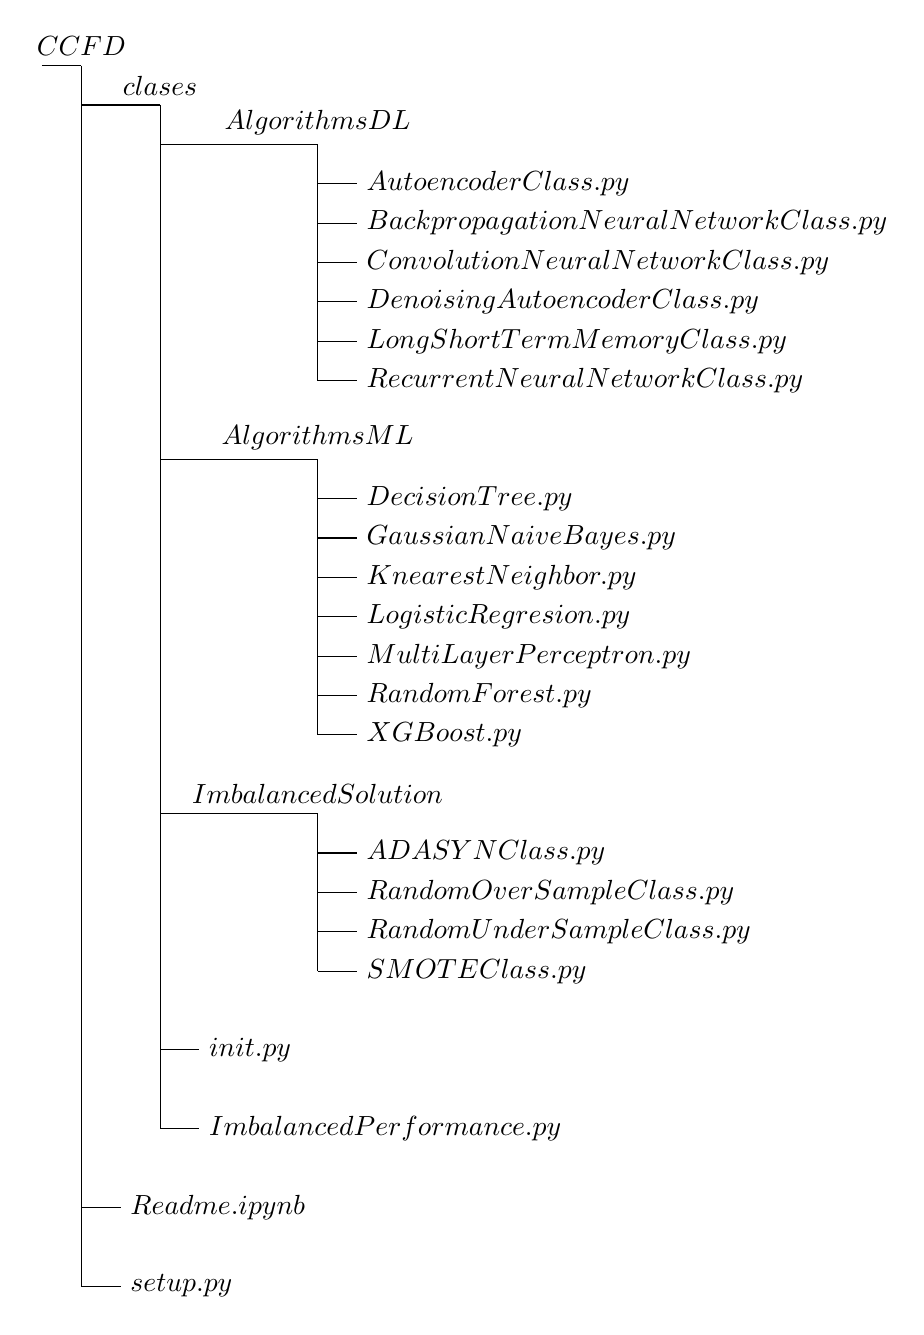
\begin{tikzpicture} % jerarqu\'{i}a de la librer\'{i}a
		% Nivel principal
		\draw (0,-0.5) -- (0.5,-0.5) node(xline1)[above]{$CCFD$};
		\draw (0.5,-0.5) -- (0.5,-1.) node(yline1)[above] {$$};
		\draw (0.5,-1) -- (0.5,-1) node(N1-1)[right] {$$};
		\draw (0.5,-1) -- (1.5,-1) node(clases)[above] {$clases$};
		\draw (0.5,-1) -- (0.5,-15) node(N1-2)[right] {$$};
		\draw (0.5,-15) -- (1,-15) node(readme)[right] {$Readme.ipynb$};
		\draw (0.5,-15) -- (0.5,-16) node(N1-3)[right] {$$};
		\draw (0.5,-16) -- (1,-16) node(setup)[right] {$setup.py$};
		% Nivel clases
		\draw (1.5,-1) -- (1.5,-1.5) node(N2-1)[right] {$$};
		\draw (1.5,-1.5) -- (3.5,-1.5) node(ADL)[above] {$AlgorithmsDL$};
		\draw (1.5,-1.5) -- (1.5, -5.5) node(N2-2)[right] {$$};
		\draw (1.5,-5.5) -- (3.5,-5.5) node(AML)[above] {$AlgorithmsML$};
		\draw (1.5,-5.5) -- (1.5, -10) node(N2-3)[right] {$$};
		\draw (1.5,-10) -- (3.5,-10) node(IS)[above] {$ImbalancedSolution$};
		\draw (1.5,-10) -- (1.5,-13) node(N2-4)[right] {$$};
		\draw (1.5,-13) -- (2,-13) node(init)[right] {$init.py$};
		\draw (1.5,-13) -- (1.5,-14) node(N2-5)[right] {$$};
		\draw (1.5,-14) -- (2,-14) node(IP)[right] {$ImbalancedPerformance.py$};
		% Nivel AlgorithmsDL
		\draw (3.5,-1.5) -- (3.5,-4.5) node(N3-1)[right] {$$};
		\draw (3.5,-2) -- (4,-2) node(AEClass)[right] {$AutoencoderClass.py$};
		\draw (3.5,-2.5) -- (4,-2.5) node(BPNNClass)[right] {$BackpropagationNeuralNetworkClass.py$};
		\draw (3.5,-3) -- (4,-3) node(CNNClass)[right] {$ConvolutionNeuralNetworkClass.py$};
		\draw (3.5,-3.5) -- (4,-3.5) node(DAEClass)[right] {$DenoisingAutoencoderClass.py$};
		\draw (3.5,-4) -- (4,-4) node(LSTMClass)[right] {$LongShortTermMemoryClass.py$};
		\draw (3.5,-4.5) -- (4,-4.5) node(RNNClass)[right] {$RecurrentNeuralNetworkClass.py$};
		% Nivel AlgorithmsML
		\draw (3.5,-5.5) -- (3.5,-9) node(N3-2)[right] {$$};
		\draw (3.5,-6) -- (4,-6) node(DT)[right] {$DecisionTree.py$};
		\draw (3.5,-6.5) -- (4,-6.5) node(GNB)[right] {$GaussianNaiveBayes.py$};
		\draw (3.5,-7) -- (4,-7) node(KNN)[right] {$KnearestNeighbor.py$};
		\draw (3.5,-7.5) -- (4,-7.5) node(LR)[right] {$LogisticRegresion.py$};
		\draw (3.5,-8) -- (4,-8) node(MLP)[right] {$MultiLayerPerceptron.py$};
		\draw (3.5,-8.5) -- (4,-8.5) node(RF)[right] {$RandomForest.py$};
		\draw (3.5,-9) -- (4,-9) node(XGB)[right] {$XGBoost.py$};
		% Nivel ImbalancedSolution
		\draw (3.5,-10) -- (3.5,-12) node(N3-3)[right] {$$};
		\draw (3.5,-10.5) -- (4,-10.5) node(ADASYN)[right] {$ADASYNClass.py$};
		\draw (3.5,-11) -- (4,-11) node(ROS)[right] {$RandomOverSampleClass.py$};
		\draw (3.5,-11.5) -- (4,-11.5) node(RUS)[right] {$RandomUnderSampleClass.py$};
		\draw (3.5,-12) -- (4,-12) node(SMOTE)[right] {$SMOTEClass.py$};
	\end{tikzpicture}
	\caption{Arquitectura de la librer\'{i}a CCFD}
	\label{ff:3}
\end{figure}

  \subsection{Componentes de las soluciones al desbalance}
    Las estrategias que se aplican en la soluci\'{o}n son las utilizadas anteriormente en los experimentos realizados. Estas estrategias est\'{a}n implementadas en la librer\'{i}a \textit{imblearn}, siendo un componente reutilizable que va a ser integrado con la librer\'{i}a \textit{sklearn} para dividir los datos en conjuntos de entrenamiento y prueba. Otro componente es \textit{pandas}, muy necesario para la lectura del conjunto de datos, en este caso de un documento \textit{Excel}. Cada componente posee una clase con las siguientes funcionalidades:
    
    \begin{align}
    	 red\_data(self,csv,test\_size=0.2)\\
    	 strategy(self)\\
    	 show\_test(self) 
    \end{align}
    
    
    La primera funcionalidad va orientada a la lectura del conjunto de datos y su divisi\'{o}n en los conjuntos de entrenamiento y prueba. Para ello recibe $csv$ como la direcci\'{o}n del archivo que almacena el conjunto de datos, y $test\_size$ como la proporci\'{o}n deseada para el conjunto de prueba con respecto al conjunto general. En la segunda funcionalidad se usa el nombre strategy como gen\'{e}rica para referirse a cada una de las estrategias dependiendo del componente. Luego de ser le\'{i}dos y particionados los datos, esta funcionalidad aplica la estrategia al conjunto de entrenamiento. Y la \'{u}ltima funcionalidad, simplemente imprime por consola los \textit{shape} de los conjuntos de entrenamiento y prueba, tanto a los que tienen aplicados la estrategia como los originales.
    
    Estos componentes permiten la obtenci\'{o}n de los conjuntos de datos de entrenamiento y prueba con estrategias aplicadas, los cuales ser\'{u}n utilizados en los modelos ML y DL.
  
  \subsection{Componentes de los modelos ML y DL}
  
    Los modelos ML seleccionados ya est\'{a}n implementados en las librer\'{i}as \textit{sklearn} y \textit{xgboost}, por lo que es un componente que ser\'{a} reutilizados. Se crea un componente por cada modelo ML utilizado en los experimentos anteriores, donde cada uno tendr\'{a} las siguientes funcionalidades:
    
    \begin{align}
    	Model(ImalancedPerformanceClass)\\
    	Modelstrategy(ImbalancedPerformanceClass)
    \end{align}
    
    Se usa Model como gen\'{e}rico para referenciar a los modelos y \textit{strategy} para referenciar a cada estrategia aplicada. \textit{ImbalancedPerformanceClass} hace referencia al componente que se explicar\'{a} despu\'{e}s, del cual extrae los conjuntos de entrenamiento y prueba de la estrategia seleccionada. En el caso de la primera funcionalidad, se devuelve una lista con un modelo por cada estrategia, siendo un total de 5, y la segunda funcionalidad, devuelve una lista con un \'{u}nico modelo dependiendo de la estrategia especificada. Cada modelo posee la siguiente estructura $(name,model,X\_train,y\_train,X\_test,y\_test)$, donde \textit{name} especifica el nombre del modelo con la estrategia, \textit{model} es el modelo, $X\_train$ y $y\_train$ es el conjunto de entrenamiento con, $y$, $X\_test$ y $y\_test$ es el conjunto de prueba.
    
    Con respecto a los modelos DL, no existe ninguna librer\'{i}a que tenga implementada las arquitecturas de los modelos seleccionados en el cap\'{i}tulo anterior. Es por ello que los componentes de cada modelo DL utiliza las mismas funcionalidades que los componentes de los modelos ML, a diferencia que en los elementos de las listas no existe \textit{model}.
  
  \subsection{Integraci\'{o}n de los componentes}
    Para la integraci\'{o}n de los componentes anteriores se desarrolla el componente \textit{ImbalancedPerformance.py}, donde mediante la clase $ImbalancedPerformanceClass$ se utilizan los componentes de soluciones al desbalance, de los modelos ML y DL, adem\'{a}s de implementar los modelos DL. Las funcionalidades que posee este componente se pueden resumir en las siguientes:
    
  \begin{align}
  	solve\_imbalanced(self,csv,test\_size=0.2)\\ 
  	performanceML(self,model)\\
  	performanceDL(self,model,dropout=[0.5,0.4,0.3])\\
  	show\_comparison(self)\\ 
  	show\_comparison\_*(self)\\
  \end{align}
  
  La primera funcionalidad se encarga de obtener todos los conjuntos de entrenamiento y prueba por cada estrategia, y almacenarlas para su pr\'{o}xima utilizaci\'{o}n. Los par\'{a}metros son los mismos que la funcionalidad $red\_data(\dots)$ de los componentes de soluciones al desbalance. La segunda funcionalidad se utiliza para realizar el entrenamiento y las pruebas, adem\'{a}s de los resultados de las m\'{e}tricas de los modelos pasados por par\'{a}metro en la variable \textit{model}, los cuales son almacenados.
  
  En la tercera funcionalidad se utiliza DL como gen\'{e}rico para referenciar a los modelos DL. A diferencia de la segunda funcionalidad, este posee el par\'{a}metro \textit{dropout}, utilizados en algunos modelos para definir el valor que tendr\'{a}n los \textit{dropouts} en esos modelos, adem\'{a}s de que se implementan los modelos. En la cuarta y quinta funcionalidad se crean \textit{Data Frames} a partir de los resultados obtenidos y almacenados de la segunda y tercera funcionalidad. El * hace referencia a variantes de la cuarta funcionalidad, donde se abarcan o difieren en algunos atributos. Esta funcionalidad devuelve dichos \textit{Data Frames}.
  
  De esta forma queda desarrollada generalmente la librer\'{i}a \textit{CCFD}, permitiendo a los usuarios realizar experimentos y pruebas a distintos conjuntos de datos.
  